
\chapter{\label{ch:proj1_LS}On the Impact of Sample Size in Reconstructing Noisy Graph Signals: General Theory \&  Least Squares Reconstruction}

\iffalse
\begin{abstract}
Reconstructing a signal on a graph from noisy observations of a subset of the vertices is a fundamental problem in the field of graph signal processing. This paper investigates how sample size affects reconstruction error in the presence of noise via an in-depth theoretical analysis of the two most common reconstruction methods in the literature, least-squares reconstruction (LS) and graph-Laplacian regularised reconstruction (GLR). Our theorems show that at sufficiently low signal-to-noise ratios (SNRs), under these reconstruction methods we may simultaneously decrease sample size and decrease average reconstruction error. We further show that at sufficiently low SNRs, for LS reconstruction we have a $\Lambda$-shaped error curve and for GLR reconstruction, a sample size of $\mathcal{O}(\sqrt{N})$, where $N$ is the total number of vertices, results in lower reconstruction error than near full observation. We present thresholds on the SNRs, $\tau$ and $\tau_{GLR}$, below which the error is non-monotonic, and illustrate these theoretical results with experiments across multiple random graph models, sampling schemes and SNRs. These results demonstrate that any decision in sample-size choice has to be made in light of the noise levels in the data.
\end{abstract}
\fi


\section{Introduction}
Real-world signals, such as brain fMRIs \cite{itani2021graph}, urban air pollution \cite{jain2014big}, and political preferences \cite{renoust2017estimating}, are often noisy and incomplete, making analysis of the signals harder. The reconstruction of these signals from limited observation is of practical importance, and can benefit from the fact that they can be treated as graph signals,  signals defined on a network domain. 
Graph signal processing (GSP) generalises the highly successful tools of sampling and reconstruction in classical signal processing by extending the classical shift operator to a graph shift operator \cite{ortega2018graph} such as the adjacency matrix \cite{EOptimalChen} or the graph Laplacian, enabling us to extrapolate the full data across the graph from observations on a subset of vertices \cite{tanaka2020sampling}. %or summaries of the data \cite{tanaka2020sampling}.

In the literature, the vast majority of studies on graph-based sampling focus on designing efficient sampling schemes that are approximately optimal under certain criteria \cite[Chapter 6]{pukelsheim2006optimal}, because optimal vertex choice under noise is in general NP-hard \cite{nikolov2022proportional, chamon2017greedy}. While \xd{these studies provide useful understanding in terms of sampling and reconstruction for graph signals, they} focus on the performance of sampling schemes at fixed sample sizes \cite{xie2019bayesian, puy2018random,shomorony2014sampling, tremblay2017determinantal,wang2018optimal,wang2019low, bai2020fast,  anis2016efficient}, while much less attention has been paid to understanding the impact of varying sample size on the mean squared error (MSE) of reconstruction. Sample size is an important parameter in both understanding and using sampling schemes, especially in the common setting of a fixed sample budget. %across all possible levels of noise, which is important for the application of graph sampling to domains such as finance \cite{nabar2023conservative} where the noise may be greater than the signal and domains where observing more samples might not be feasible and subsampling is more feasible.

\begin{table}[ht]
    \centering
    \caption{Studies on the Impact of Sample Size on MSE}
    \begin{subtable}[h]{\linewidth}
        \centering
        \begin{tabularx}{\linewidth}{lp{2cm}Xp{4cm}}
            \toprule
            \textbf{Reference} & \textbf{Considers Noise?} & \textbf{Reconstruction Method} & \textbf{Range of Possible Sample Sizes} \\
            \midrule
            Tremblay, 2017 \cite{tremblay2017determinantal} & \checkmark & LS, GLR & Limited \\
            Wang, 2018 \cite{wang2018optimal} & \checkmark & LS & Limited \\
            Wang, 2019 \cite{wang2019low} & \checkmark & LS & Limited \\
            Bai, 2020 \cite{bai2020fast} & \checkmark & GLR & Limited \\
            Anis, 2016 \cite{anis2016efficient} & \checkmark & LS & Full \\
            \bottomrule
        \end{tabularx}
        \caption{Empirical Results}
    \end{subtable}
    
    \vspace{1em}
    
    \begin{subtable}[h]{\linewidth}
        \centering
        \begin{tabularx}{\linewidth}{lp{2cm}Xp{4cm}}
            \toprule
            \textbf{Reference} & \textbf{Considers Noise?} & \textbf{Reconstruction Method} & \textbf{Range of Possible Sample Sizes} \\
            \midrule
            Puy, 2018 \cite{puy2018random} & \checkmark & LS & Limited \\
            Chamon, 2017 \cite{chamon2017greedy} & \checkmark & LS (Regularised) & Full \\
            Shomorony, 2014 \cite{shomorony2014sampling} & \texttimes & LS & Full \\
            \textbf{Chapter \ref{ch:proj1_LS}} & \textbf{\checkmark} & \textbf{LS} & \textbf{Full} \\
            \textbf{Chapter \ref{ch:proj1_GLR}} & \textbf{\checkmark} & \textbf{GLR} & \textbf{Full} \\
            \bottomrule
        \end{tabularx}
        \caption{Theoretical Results}
    \end{subtable}
    \label{tbl:Lit_review}
\end{table}

The literature studies the impact of sample size both empirically and theoretically \bs{(summarised in Table \ref{tbl:Lit_review})}, and can be further divided by the setting considered: whether the observations are noisy or noiseless, and by which reconstruction method. Empirical results, linked to sampling schemes, are usually obtained in the noisy setting under least squares (LS) reconstruction or its variants \cite{ tremblay2017determinantal,wang2018optimal,wang2019low,chamon2017greedy} or graph-Laplacian regularised (GLR) reconstruction \cite{bai2020fast, tremblay2017determinantal}. These results show that MSE decreases as sample size increases in a restricted range of noise level and sample size. An exception is \cite[Fig. 1]{anis2016efficient} which empirically shows non-monotonicity of MSE with sample size under LS as it considers the {\color{black}full range of possible sample sizes, including sample sizes less than bandwidth,} and a relatively high noise level. Of the three main theoretical results on the impact of sample size in the literature, two focus on slightly different settings: \cite{shomorony2014sampling} presents sample size bounds for perfect signal reconstruction in the noiseless setting, while \cite[\bs{Lemma 1}]{chamon2017greedy} proves that MSE decreases as sample size increases in the noisy setting and provides bounds on the impact of sample size on MSE, but assumes a specific form of regularised LS which is Bayesian optimal. While these theoretical results provide valuable insight, the settings they are based on do not always agree with those in the empirical studies above, hence a generic understanding is still lacking. The third theoretical result \cite[Theorem 6]{puy2018random} assumes unregularised LS and noisy reconstruction, and proves an MSE upper bound that is tight and decreasing in sample size; however, this result is practically constrained to the case where sample size is greater than or equal to bandwidth \cite[Eq. 3]{puy2018random}.
%can give insight to the impact of MSE, as they are in a different setting to the empirical results they do not apply in that setting.

In this chapter, we fill the gap in the literature by providing a theoretical characterisation of the impact of sample size on \bs{the average} MSE \bs{ (or MMSE  -- see Section \ref{sec:Optimality_Criteria})} across the full range of possible sample sizes in the most common settings, i.e. noisy observations and LS or GLR reconstruction. More specifically, we focus on whether under sufficiently low SNRs, decreasing sample size may actually decrease MSE. Furthermore, we investigate both the full range of sample sizes and all possible levels of noise, which is important for the application of graph sampling to domains where the noise may be greater than the signal \xd{(e.g. finance, with typically low signal-to-noise ratio \cite{nabar2023conservative}, or environmental sciences,  with inaccurate measurements from low-cost sensors \cite{bush2023impact})} or when observing more samples might not be feasible (e.g. resource-constrained settings). This breadth is only possible through our rigorous theoretical characterisation which allows us to understand behaviour at high noise levels\bs{,} to characterise behaviour on arbitrarily large graphs\bs{,} and to show when certain behaviours of MSE happen and why. %While theorems often need to be narrow in scope to allow for tractable proofs, our results are notable in how loose their restrictions are; our results for LS reconstruction apply to all graphs and every determinstic sampling scheme in the literature, while the conditions of our main result for GLR reconstruction under full-band noise, empirically, hold for every Erdős–Rényi, Stochastic Blockmodel and Barabasi-Albert graph tested (Table \ref{tbl:empirical_probabilities_conditions}).

Our results begin by using a Bias-Variance decomposition to explain why decreasing sample size may decrease MSE for any linear reconstruction method \xd{(Section \ref{sec:general})}, and we then specialise to LS and GLR \bs{(Section \ref{sec:every_x})}. We prove that under LS reconstruction of a $k$-bandlimited signal, if the samples were chosen to be optimal in the noiseless case then we can always reduce MSE under high noise by reducing sample size from $k$ to $k-1$ {\color{black}(Section \ref{sec:LS_full_band}, Theorem \ref{thm:noiseless_optimality_means_noise_sensitivity})}. We prove that under GLR, if certain graph invariants hold on a graph with $N$ vertices, reducing sample size from almost $N$ vertices to $\mathcal{O}(\sqrt{N})$ vertices will reduce MSE at high noise levels {\color{black}(Section \ref{sec:GLR_full_band}, Proposition \ref{propn:GLR_simple})}, and that these invariants hold for large Erdős–Rényi graphs with high probability {\color{black}(Section \ref{sec:GLR_full_band}, Proposition \ref{propn:GLR_big_N})}. Our experiments {\color{black}(Section \ref{sec:experiments})} validate this for {\color{black} large} Stochastic Blockmodel and Barabasi-Albert graphs as well, {\color{black} demonstrating the applicability of our results to graphs with community structure and large scale-free networks}. We also investigate how sensitive our results are to different kinds of noise by presenting variants of our theoretical and empirical results under both bandlimited \bs{(Sections \ref{sec:LS_bandlimited}) \& \ref{sec:GLR_bandlimited}} and full-band noise \bs{(Sections \ref{sec:LS_full_band} \& \ref{sec:GLR_full_band})}. \xd{Although our results are mainly of theoretical nature, they may provide useful guidance on choosing the appropriate sample size in light of noise levels in the data.}

Our paper presents four primary contributions: 
\begin{enumerate}
    \item A theoretical characterisation of how decreasing sample size may decrease MSE, not only under LS  but also under GLR, a regularised method. 
    \item Analysis of both LS and GLR under bandlimited noise to show non-monotonicity of the MSE is not caused by just the high frequency component of the noise.
    \item Asymptotic analysis, showing how the non-monotonicity of the MSE with sample size persists as $N \to \infty$.
    \item Extensive experimental simulations illustrating the theoretical results under LS and GLR, and bandlimited noise.
\end{enumerate}
The present work is a significant extension of a previous conference paper \cite{sripathmanathan2023impact}, where
preliminary versions of Corollary \ref{main_ls}, Proposition \ref{propn:main_existence_LS}, and a weaker version of Theorem \ref{thm:noiseless_optimality_means_noise_sensitivity} were presented, corresponding to the LS part of contribution 1) above. 
Lemmas \ref{lemma:LS_xi_1_is_rank}-\ref{lemma:LS_delta_1_improvement_means_delta_2_worse} closely follow those in the conference version \cite{sripathmanathan2023impact}.


\section{Background \& Problem Formulation}

\xd{In this section, we first introduce basic definitions of graphs, and the signal and noise models we focus on. We then provide notations for sampling, discuss reconstruction methods, and evaluation criteria. 
% In this section, we first introduce basic graph definitions and sampling notation. We then discuss graph signal reconstruction in three parts: what we reconstruct (graph signals), how we reconstruct them (reconstruction methods), and how the reconstruction is evaluated (optimality criteria). 
Finally, we present our problem setting.}

\subsection{Graphs and Graph Signals}
\label{sec:signal_model}
A graph $\set{G}$ consists of a set of $N$ vertices, a set of edges between these vertices, and the associated edge weights. We assume $\mathcal{G}$ is connected and undirected, and that the combinatorial graph Laplacian $\matr{L}$ is real positive semidefinite with $N$ distinct eigenvalues $0 = \lambda_{1} < \lambda_{2} < \ldots < \lambda_{N}$ which are also called \emph{graph frequencies} \cite{ortega2018graph}\footnote{Although we focus on the combinatorial graph Laplacian, our results on LS also hold for the normalised graph Laplacian or any graph shift operator that is positive semidefinite.}. {\color{black}Write the eigendecomposition of $\matr{L}$ as $\matr{L} = \matr{U}\matr{\Lambda}\matr{U}^{T}$ where $\matr{\Lambda} = diag(\lambda_{1},\ldots,\lambda_{N})$ and the columns of $\matr{U}$ are the eigenbasis of $\matr{L}$ and form an orthonormal basis of $\mathbb{R}^{N}$.
\iffalse
\begin{equation}
    \matr{L} = \matr{U} \begin{pmatrix}
        \lambda_{1} & & \matr{0} \\
        & \ddots & \\
        \matr{0} & & \lambda_{N}
    \end{pmatrix}\matr{U}^{T}
\end{equation}
where the columns of $\matr{U}$ are the eigenbasis of $\matr{L}$ and form an orthonormal basis of $\matr{R}^{N}$.
\fi

}
%\subsection{Graph Signals}
The most common signal model used in the graph signal processing literature is the bandlimited signal model, where a $k$-\emph{bandlimited signal} is a linear combination of the first $k$ columns of $\matr{U}$\cite{EOptimalChen}. This is a common smoothness model for graph signals. To obtain this, \bs{we define $\projbl$ as the projection operator that $k$-bandlimits a signal (we provide a symbolic definition in Section \ref{sec:notation}).}
%To facilitate our discussion we first introduce a few handy notations.

%Sec II.B

%We can understand $\projbl$ as converting a signal into the nearest $k$-bandlimited signal.  %, and the space of such signals is called a Paley-Wiener space \cite{pesenson2008sampling}.%, written either as $PW_{\omega}(\mathcal{G})$ for any $\omega \in [\lambda_{k}, \lambda_{k+1})$ or $\text{BL}_{k}(\matr{U}^{T})$ \cite{EOptimalChen}.

It is rare for observed signals to be perfectly bandlimited{\color{black}. While this can be modelled by assuming the underlying signal to be reconstructed is not bandlimited but rather} `approximately bandlimited signals'\cite{chen2016signal, lin2019active}, or from other more general priors \cite{tanaka2020generalized, hara2022sampling}, we take the more \bs{common approach \cite{wang2018optimal, wang2019low,bai2020fast, puy2018random, tremblay2017determinantal}} of assuming {\color{black}the underlying signal is $k$-bandlimited} with additive observation noise. We assume we observe a corrupted signal $\vect{y} = \vect{x} + \vect{n}$ %at a subset of the vertices $\set{S}$ 
where
\begin{itemize}
    \item $\vect{x}$ is a random $k$-bandlimited signal with $\expect{\vect{x}} = 0$ and $\text{Cov}(\vect{x}) = \projbl$,
    \item $\vect{n} = \sigma \cdot \vect{\epsilon}$ is noise where $\sigma > 0$, $\expect{\vect{\epsilon}} = 0$ and either
    {\color{black}
    \begin{enumerate}
        \item $\text{Cov}(\vect{\epsilon}) = \matr{I}_{N}$ (`full-band noise')
        \item $\text{Cov}(\vect{\epsilon}) = \projbl $  (`$k$-bandlimited noise')
    \end{enumerate}
    }
\end{itemize}
{\color{black} Our results apply to any noise with these properties (e.g. Gaussian or Rademacher noise).}
We refer to the $\text{Cov}(\vect{\epsilon}) = \matr{I}_{N}$ case as `full-band noise' as the associated corrupted signal $\vect{y}$ has high frequency components, whereas the other case does not. In the literature, noise levels are often described using the SNR = $\frac{\expect{\sqnormvec{ \vect{x} }}}{\expect{\sqnormvec{\vect{n}}}}$, {\color{black} a ratio of norms which must be positive\footnote{It is common in the literature to express the SNR in decibels, which may be negative, while its ratio form remains positive. We will use the ratio form unless otherwise noted, so for example $-20dB$ will be written as $10^{-20/10}  > 0$.}. We note that under full-band noise we have $\sigma^{2} = \frac{k}{N \cdot \text{SNR}}$ and under $k$-bandlimited noise we have $\sigma^{2} = \frac{1}{\text{SNR}}$.} 

\iffalse
{\color{black} We now briefly discuss and motivate our choice of signal and noise model. The main result -- that decreasing sample size can decrease MSE -- is not fundamentally dependent on the signal model for $\vect{x}$, and does not even require bandlimitedness of $\vect{x}$. This is discussed in depth in Section \ref{sec:general}. We choose $k$-bandlimited signals to mirror the setup found in the related sampling literature CITECITECITE.

Our results are dependent on the noise model and thus we look at two specific noise models, which shows that our results are not totally intertwined with a specific choice of noise covariance. The full-band noise model is commonly found in the literature. The $k$-bandlimited noise model has noise related to the graph, and is thus of theoretical interest. %which is a property frequently found in practice.   
}
\fi

\subsection{Notation for Sampling}
\label{sec:notation}
We use the same submatrix notation as \cite{zhang2000schur}.  For any matrix $\matr{X}$ and sets $\set{A},\set{B}$, we write $\matrsub[A,B]{X}$ to be the submatrix of $\matr{X}$ with row indices in $\set{A}$ and column indices in $\set{B}$. We define the subvector $\vectsub[A]{x}$ of a vector $\vect{x}$ similarly. We define a specific shorthand for taking a principal submatrix:
\begin{equation}
    \matrsub[A]{X} = \matrsub[A,A]{X}.
\end{equation}
We let $\set{N} = \{1, \ldots, N\}$ and $\set{K} = \{1, \ldots, k\}$. We also define two pieces of notation for projections. Let
\begin{align}
    \proj{B} &= \matrsub[N,B]{I}\matrsub[B,N]{I},   &
    \projbl &= \matrsubU{N}\matrsubU{N}^{T}.
\end{align}
Finally, $\set{A} \backslash \set{B} = \{ i \in A \, \mid \, i \notin B \} $ and $\set{A}^{c} = \set{N} \backslash \set{A}$. In general, we adhere to standard set notation.

{\color{black} We will mainly use $\set{N}$ to index the vertices of $\set{G}$ and use $\set{K}$ to index the first $k$ columns of $\matr{U}$. $\projbl$ can be understood as an ideal low-pass filter.}

\subsection{Reconstruction Methods}
We define a \emph{reconstruction method} (or `interpolation operator' \cite{chamon2017greedy}) to take potentially noisy observations on a vertex sample set $\set{S}$ and reconstruct the signal across all vertices. In this paper we focus on LS and GLR, \bs{and we present their objectives here:
\begin{flalign}
        &\text{LS:} \hspace{0.13\columnwidth}  \hat{\vect{x}} =  \argmin_{\vect{x} \in \text{span}(\matrsubU{N})} || \vectsub[S]{x} - \vect{y} ||_{2}   & \label{eq:LS_Defn} \\ 
        &\text{GLR:} \hspace{0.1\columnwidth}  \hat{\vect{x}} = \hspace{11pt} \argmin_{\vect{x} \in \mathbb{R}^{N}}  \sqnormvec{ \vectsub[S]{x} - \vect{y}} + \mu \vect{x}^{T}\matr{L}\vect{x} & \label{eq:GLR_Defn}
\end{flalign}
}
We summarise their differences in Table \ref{tab:tbl1}, labelling the input parameters into the reconstruction, whether they are biased and whether they require computation of the {\color{black}eigenbasis} $\matrsubU{N}$. 

\iffalse
\begin{table}[h]
\caption{The LS and GLR reconstruction Methods.}    \renewcommand*{\arraystretch}{1.5}

\begin{center}
    \begin{tabularx}{(\textwidth - 12pt)/2}{| @{\hspace{0.1cm}}p{0.4cm} | @{\hspace{0.1cm}}p{4.45cm} |@{\hspace{0.1cm}}p{0.65cm}| @{\hspace{0.1cm}}p{0.7cm}|@{\hspace{0.1cm}}X|}
    \hline
      & \thead{Objective} & \textbf{Param} & \textbf{Biased} & \textbf{Needs } $\matrsubU{N}$ \\
    \hline
        LS  & $\displaystyle \hat{\vect{x}} =  \argmin_{\vect{x} \in \text{span}(\matrsubU{N})} || \vectsub[S]{x} - \vect{y} ||_{2}$ & $k$ & no & yes \\
        \hline
        GLR & $\displaystyle \hat{\vect{x}} = \argmin_{\vect{x} \in \mathbb{r}^{n}}  \sqnormvec{ \vectsub[s]{x} - \vect{y}} + \mu \vect{x}^{t}\matr{l}\vect{x} $ & $\mu$ & yes & no \\
        \hline
    \end{tabularx}
\end{center}
\label{tab:tbl1}
\end{table}
\fi

\begin{table}[h]
\caption{The LS and GLR reconstruction Methods.}
\renewcommand*{\arraystretch}{1.5}
\centering
\begin{tabular*}{\textwidth}{l@{\extracolsep{\fill}}ccc}
    %\begin{tabular}{lccc}
    \toprule
      & \textbf{Parameters} & \textbf{Biased} & \textbf{Requires Computing $\matrsubU{N}$} \\
    \midrule
        LS  & $k$ & $\times$ & $\checkmark$ \\
        GLR  & $\mu$ & $\checkmark$ & $\times$ \\
    \bottomrule
    \end{tabular*}
\label{tab:tbl1}
\end{table}

Our analysis of LS also applies to the commonly used iterative reconstruction method, Projection onto Convex Sets \cite{narang2013localized}, as POCS converges to LS.

We call a reconstruction method \emph{linear} if it is linear in its observations. For a fixed vertex sample set $\set{S}$ we can represent a linear reconstruction method by a matrix $\matr{R}_{\set{S}} \in \mathbb{R}^{N \times |\set{S}|}$.

\begin{remark}
    LS and GLR are both linear:
    \begin{align}
    \textrm{LS:\quad} \matr{R}_{\set{S}} &= \matrsubU{N}\matrsubU{S}^{\dagger} \label{eq:defn_RS:LS}\\
    \textrm{GLR:\quad} \matr{R}_{\set{S}} &= \msub[N,S]{( \proj{S} + \mu \matr{L})^{-1}} \label{eq:defn_RS:GLR}
    \end{align}
\end{remark}
\noindent where for a matrix $\matr{A}$, $\matr{A}^{\dagger}$ is its Moore-Penrose pseudoinverse.

Across all linear models under the noisy setting, LS leads to the minimum-variance unbiased estimator of $\vect{x}$ \cite{gauss1823theoria} {\color{black} for $k$-bandlimited signals and full-band noise}, which theoretically justifies us focusing our analysis on LS. 
\bs{}On the other hand, GLR implicitly assumes a multivariate Gaussian signal with covariance $\matr{L}^{\dagger}$\cite{dong2016learning}, which is slightly mismatched with the $k$-bandlimited signal model we focus on in this paper. Nevertheless, in practice GLR is still often used for large graphs as computing $\matrsubU{N}$ for LS is slow \cite{puy2018random, bai2020fast}. It is also a typical regression model that promotes signal smoothness and has been widely adopted in the literature \cite{belkin2004semi}. Because of these considerations we believe GLR is still a meaningful case to study.

Finally, we clarify what we mean when we consider LS with sample size less than bandwidth. {\color{black} In this case }if LS is defined as the minimisation of the objective \bs{(\ref{eq:LS_Defn})} there are multiple solutions. Thus, we follow \cite{anis2016efficient} and define the LS reconstruction as the 
unique minimum-norm solution \cite[Sect. 5.5.1]{golub13}, hence (\ref{eq:defn_RS:LS}) applies regardless of sample size. 

{\color{black}
\begin{remark}    
We note that if $\vect{x}, \vect{\epsilon}$ and $\sigma$ are Gaussian, we can compute the best predictor of $\vect{x}$ in MSE terms. This is the expectation of $\vect{x}$ conditional on the observation, and is also known as the `Optimal Bayesian Reconstruction'. It has been proven in this case that decreasing sample size must increase MSE \cite{chamon2017greedy}. We do not attempt to characterise this or other noise-adaptive methods; we assume that $\matr{R}_{\set{S}}$ is not dependent on $\sigma$.
\end{remark}
}

 
\subsection{Optimality Criteria for Sampling}
\label{sec:Optimality_Criteria}
To meaningfully contrast choices of vertex sample set size and selection, we need to evaluate reconstruction performance, and we do so by certain optimality criteria. In the noiseless case, the main optimality criterion for a vertex sample set $\set{S}$ is whether it is a \emph{uniqueness set} 
 \cite{pesenson2008sampling}, that is, if we can perfectly reconstruct any $k$-bandlimited signal observed on $\set{S}$. Such a set always exists and $\set{S}$ is a uniqueness set for a bandwidth $k$ if and only if $\text{rank}(\matrsubU{S}) = k$ \cite{anis2016efficient}. 
 
 In the case of additive observation noise, there are multiple common optimality criteria \cite[Chapter 6]{pukelsheim2006optimal}:

\begin{itemize}
    \item \emph{MMSE criterion}: Minimise  average MSE. \cite{wang2018optimal,wang2019low, mfn}
    \item \emph{Confidence Ellipsoid criterion}: Minimise the confidence ellipsoid around the eigenbasis co-efficients. \cite{jayawant2021doptimal, tremblay2017determinantal, mfn}
    \item \emph{WMSE criterion}: Minimise worst-case MSE. \cite{bai2020fast, EOptimalChen}
\end{itemize}

\noindent 
Under LS, these criteria have the following names and forms:
\begin{align}
    \text{\emph{(MMSE)} A-Optimality:} &\text{ minimise } \text{tr}(\matr{P}^{-1}) \label{eq:A-optimality}\\
    \text{\emph{(Conf. Ellips.)} D-Optimality:} &\text{ maximise } \text{det}(\matr{P})
 \label{eq:D-optimality}\\
    \text{\emph{(WMSE)} E-Optimality:} &\text{ maximise }
        \lambda_{min}(\matr{P}) \label{eq:E-optimality}
\end{align}
%\noindent where $\matr{P}$ is defined as %where $\lambda_{min}(\matr{P})$ is the minimum eigenvalue of $\matr{P}$ defined as: %\in \mathbb{R}^{d \times d}$,
\begin{flalign}
    &\text{where }&\matr{P} = \begin{cases}
        \projbl[S] &\text{if }|\set{S}| < k \\
        \matrsubU{S}^{T}\matrsubU{S} &\text{if }|\set{S}| \geq k
    \end{cases} \qquad\qquad\qquad&
\end{flalign}  

\noindent and we define $\trace{\matr{P}^{-1}} = +\infty$ in (\ref{eq:A-optimality}) if $\matr{P}$ is not invertible.

\subsection{Problem Setting}
In this paper, we are interested in a theoretical characterisation of the impact of sample size on MSE under all possible SNRs. 
For our theoretical results and experiments, we assume:
\begin{itemize}
    \item A known graph $\mathcal{G}$ which is connected and undirected.
    \item A known bandwidth $k$.
    \item A clean underlying $k$-bandlimited signal $\vect{x}$ drawn from a known distribution.
    \item Observations of $\vect{x}$ are corrupted by noise which is either:
    \begin{itemize}
        \item full-band, so we observe a non-bandlimited signal.
        \item $k$-bandlimited, so we observe a $k$-bandlimited signal.
    \end{itemize}
    \item Linear reconstruction, in particular LS and GLR.
\end{itemize}
In this paper, we study the behaviour of the MMSE criterion, that is, the MSE averaged over a known signal model and known noise model, which we write as
\begin{equation}
    \textrm{MSE}_{\set{S}} = \expect[\vect{x},\vect{\epsilon}]{\sqnormvec{\hat{\vect{x}} - \vect{x}} \smallskip \mid \set{S} \textrm{ observed} }.
\end{equation}
\iffalse
{\color{black} While it is not the focus, we note that all results in this paper extend to any finite-variance signal model for $\vect{x}$, including the fixed $\vect{x}$ case; we discuss this in Section \ref{sec:general}.
}
\fi

\section{Main {\color{black}Theoretical} Results}
\label{main_results_sec}
\subsection{Overview and Proof Approaches}
\label{sec:theory-overview}
In this section, we prove theorems showing how the relationship between sample size and MSE changes with different levels of observation noise, with a focus on showing when reducing sample size reduces MSE. We first present a high level sketch of our approach. To study the effect of noise, we perform a Bias-Variance decomposition on the MSE:
\begin{equation}
    \textrm{MSE}_{\set{S}} = \underbrace{\xi_{1}(\set{S})}_{\expect{\text{bias}^{2}}} + \underbrace{\sigma^{2} \cdot \xi_{2}(\set{S})}_{\expect{\text{variance}}} 
\end{equation}
where the bias term $\xi_{1}(\set{S}) = \text{MSE}_{\set{S}}$ when $\sigma^{2} = 0$ is the MSE attributable to reconstruction of the clean signal, and $\xi_{2}(\set{S})$ can be understood as a sensitivity-to-noise term (see Section \ref{sec:general} for derivations).
With this decomposition, the relationship between sample size and MSE under different levels of noise reduces to how the bias and sensitivity-to-noise vary with respect to sample size. 

The focus of the paper is not to characterise all the cases where decreasing sample size decreases MSE, but rather to clearly show that it does happen in a wide variety of cases. In service of this, we focus on certain broad cases that are more tractable, which we call `simplifications'. For example, we only compare a sample set $\set{S}$ to a subset of it, i.e., $\set{T} \subset \set{S}$.

\begin{mccorrection}
Our general approach per reconstruction method is described in Figure \ref{fig:theory_structure_flowchart}:
\end{mccorrection}
\iffalse
\begin{itemize}
    \item Choose a simplification (`simplify');
    \item Under this simplification, characterise all conditions when decreasing sample size can decrease MSE (`characterise');
    \item Show that these conditions actually happen (`existence');
    \item Study these conditions as $N \to \infty$, to prove the conditions may happen on large graphs (`asymptotics').
\end{itemize}
\fi

\begin{figure}[htbp]
    \centering
    % reconstruction_flowchart.tikz
% Styles
\tikzstyle{startstop} = [rectangle, rounded corners, minimum width=3cm, minimum height=1cm, text centered, draw=black, align=center]
\tikzstyle{process} = [rectangle, minimum width=3cm, minimum height=1cm, text centered, draw=black, align=center]
\tikzstyle{arrow} = [thick,->,>=stealth]

% Flowchart
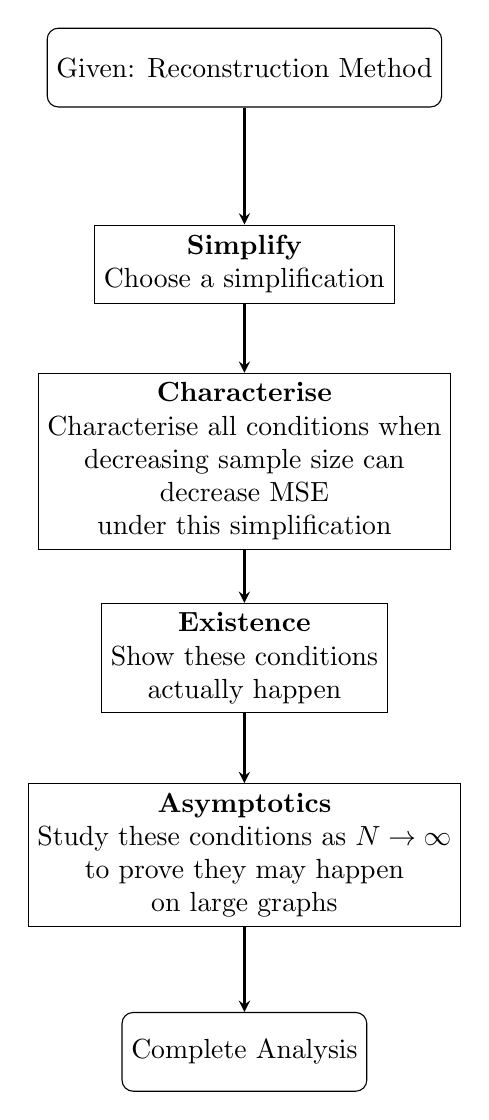
\begin{tikzpicture}[node distance=2.5cm]

% Define nodes
\node (start) [startstop] {Given: Reconstruction Method};
\node (simplify) [process, below of=start] {{\bf Simplify}\\Choose a simplification};
\node (characterise) [process, below of=simplify] {{\bf Characterise}\\Characterise all conditions when\\decreasing sample size can\\decrease MSE \\ under this simplification};
\node (existence) [process, below of=characterise] {{\bf Existence}\\Show these conditions\\actually happen};
\node (asymptotics) [process, below of=existence] {{\bf Asymptotics}\\Study these conditions as $N \to \infty$\\to prove they may happen\\on large graphs};
\node (end) [startstop, below of=asymptotics] {Complete Analysis};

% Draw arrows
\draw [arrow] (start) -- (simplify);
\draw [arrow] (simplify) -- (characterise);
\draw [arrow] (characterise) -- (existence);
\draw [arrow] (existence) -- (asymptotics);
\draw [arrow] (asymptotics) -- (end);

\end{tikzpicture}
    \caption{\mccorrect{General approach for reconstruction methods}}
    \label{fig:theory_structure_flowchart}
\end{figure}


For LS, we simplify the problem by only considering decreasing the sample size by one at a time, which we call the `single vertex' simplification. We pay particular attention to subsets sampled by sampling schemes that are optimal in the noiseless setting (Subsection \ref{sec:LS_full_band}). For GLR, we compare observing the full graph to observing a subset of the vertices. We call this the `full observation' simplification. We focus on graphs which satisfy certain graph invariants (Subsection \ref{sec:GLR_full_band}). We justify these simplifications in the relevant subsections below.
 
We then consider reconstruction under bandlimited noise (Subsections \ref{sec:LS_bandlimited} and \ref{sec:GLR_bandlimited}) to show that the reduction in MSE from reducing sample size is not sensitive to our noise model, nor due to the high frequency component of the noise.

\xd{An overview of the four steps in our general approach together with the main results are summarised in Table \ref{tbl:general_theory}.}

\iffalse
\begin{table}[h]
{\color{black}
\caption{Structure of Theoretical Results}
\centering
\begin{tabularx}{(\textwidth - 12pt)/2}{| @{\hspace{0.1cm}}p{0.8cm} | @{\hspace{0.1cm}}X | @{\hspace{0.1cm}} >{\centering\arraybackslash} p{1.25cm} | @{\hspace{0.1cm}}p{1.4cm} | @{\hspace{0.1cm}}p{1cm} | @{\hspace{0.1cm}}X |}
\hline
 &  & Step 1: & Step 2: & Step 3: & Step 4: \\
 & \emph{Noise} & \emph{Simplification} & \emph{Characterisation} & \emph{Existence} & \emph{Asymptotics} \\
\hline
General & Any & $\set{S} \supset \set{T} $ & Thm \ref{main_general} & &\\ \hline
\multirow{2}{*}{LS} & Full-band  & \multirow{2}{*}{$\set{S}$ vs $\set{S}\backslash \{v\}$} & Corr \ref{main_ls} & Thm \ref{thm:noiseless_optimality_means_noise_sensitivity} & Remark \ref{rmk:LS_big_N}\\ 
 & Bandlimited &  & Corr \ref{corr:LS_bandlimited_noise_big_variance} & Corr \ref{corr:LS_bandlimited_noise_sample_only_k}&Remark \ref{rmk:LS_big_N_bl}\\\hline
\multirow{2}{*}{GLR} & Full-band & \multirow{2}{*}{$\set{N}$ vs $\set{S}$}& \multirow{2}{*}{Corr \ref{corr:main_GLR_iff}} & Thm \ref{thm:main_GLR_exist} & Propn \ref{propn:GLR_big_N}\\ 
 & Bandlimited & &  & Thm \ref{thm:main_GLR_bl} & Propn \ref{propn:GLR_big_N_bl}\\
\hline
\end{tabularx}
\label{tbl:general_theory}
}
\end{table}
\fi 
\iffalse
\begin{table}[h]
\caption{Structure of Theoretical Results}
\centering
\begin{tabularx}{\linewidth}{|@{\hspace{0.1cm}}p{2.4cm}|X|p{1.8cm}|p{2.4cm}|p{1.8cm}|p{2.4cm}|}
\hline
 & General &\multicolumn{2}{c|}{LS} & \multicolumn{2}{c|}{GLR} \\
\hline
{Noise} & Any & Full-band & Bandlimited & Full-band & Bandlimited \\
\hline
\emph{Simplification} & $\set{S} \supset \set{T}$ & \multicolumn{2}{c|}{$\set{S}$ vs $\set{S} \backslash \{v\}$} &  \multicolumn{2}{c|}{$\set{N}$ vs $\set{S}$}  \\
\hline
\emph{Character- isation} & Thm \ref{main_general} & Corr \ref{main_ls} & Corr \ref{corr:LS_bandlimited_noise_big_variance} & \multicolumn{2}{c|}{Corr \ref{corr:main_GLR_iff}}  \\
\hline
\emph{Existence} & & Thm \ref{thm:noiseless_optimality_means_noise_sensitivity} & Corr \ref{corr:LS_bandlimited_noise_sample_only_k} & Thm \ref{thm:main_GLR_exist} & Thm \ref{thm:main_GLR_bl} \\
\hline
\emph{Asymptotics} & & Remark \ref{rmk:LS_big_N} & Remark \ref{rmk:LS_big_N_bl} & Propn \ref{propn:GLR_big_N} & Propn \ref{propn:GLR_big_N_bl} \\
\hline
\end{tabularx}
\label{tbl:general_theory}

\end{table}
\fi


\begin{table}[h]
\caption{Structure of Theoretical Results}
\centering
\begin{tabular}{@{} l >{\centering\arraybackslash}p{6em}  c c @{}}
\toprule
 & General & \multicolumn{2}{c}{LS} \\
\cmidrule(lr){3-4}
{} & Any Noise & Full-band Noise & Bandlimited Noise \\
\midrule
\emph{Simplification} & $\set{S} \supset \set{T}$ & {$\set{S}$ vs $\set{S} \backslash \{v\}$} & {$\set{S}$ vs $\set{S} \backslash \{v\}$} \\
\midrule
\emph{Characterisation} & Thm \ref{main_general} & Corr \ref{main_ls} & Corr \ref{corr:LS_bandlimited_noise_big_variance} \\
\midrule
\emph{Existence} & & Thm \ref{thm:noiseless_optimality_means_noise_sensitivity} & Corr \ref{corr:LS_bandlimited_noise_sample_only_k} \\
\midrule
\emph{Asymptotics} & & Remark \ref{rmk:LS_big_N} & Remark \ref{rmk:LS_big_N_bl} \\
\bottomrule
\end{tabular}
\label{tbl:general_theory}
\end{table}



%\bs{Our theoretical results for $k$-bandlimited noise can be found in Appendix \ref{app:LS_bandlimited} for LS and Appendix \ref{app:GLR_bandlimited} for GLR.}

\subsection{General Results}
\label{sec:general}
{\color{black}








We start with general results. All results in this Section \ref{sec:general} apply to a very general signal model; we only assume that $\vect{x}$ and $\vect{\epsilon}$ are drawn from independent distributions, that $\expect{\vect{\epsilon}} = 0$, $\expect{\sqnormvec{\vect{x}}} < \infty$ and $\expect{\sqnormvec{\vect{\epsilon}}} < \infty$ . We then specialise to the signal and noise models introduced in Section \ref{sec:signal_model}, based on which we present the analysis in Section \ref{sec:every_x} and results in Sections \ref{sec:LS_full_band}, \ref{sec:GLR_full_band}, \ref{sec:LS_bandlimited} and \ref{sec:GLR_bandlimited}.

To understand the effect of changing the sample size on MSE at different levels of noise, we use a variant of the Bias-Variance decomposition  \cite{geman1992neural} on the MSE to separate out the effect of noise. Let $\hat{\vect{x}}$ be a reconstruction of the signal $\vect{x}$, then
\begin{equation}
    \textrm{MSE}_{\set{S}} = \expect[\vect{x}]{\underbrace{\sqnormvec{\vect{x} - \expect[\vect{\epsilon}]{\hat{\vect{x}}}}}_{\text{Bias}(\hat{\vect{x}},\vect{x})^{2}} + \underbrace{\expect[\vect{\epsilon}]{\sqnormvec{ \expect[\vect{\epsilon}]{\hat{\vect{x}}} - \hat{\vect{x}}}}}_{\text{Var}(\hat{\vect{x}})}} \label{eq:Bias_var_decomp_general}
\end{equation}
This decomposition applies to \emph{any} reconstruction $\hat{\vect{x}}$ of $\vect{x}$.
\begin{proof}
    See Appendix \ref{app:bias-variance} or \cite[Chapter 5.4.4]{Goodfellow2016DeepLearning}.
\end{proof}
}
We consider reconstructing a signal with a linear reconstruction method. We first consider a generic $\matr{R}_{\set{S}}$. 
\noindent For linear reconstruction, we have $\hat{\vect{x}} = \matr{R}_{\set{S}}\vectsubgen[\set{S}]{\vect{x} + \sigma \cdot \vect{\epsilon}}$. By assumption, $\expect{\vect{\epsilon}} = 0$, so $\expect[\vect{\epsilon}]{\hat{\vect{x}}} = \matr{R}_{\set{S}}\vectsub[S]{x}$. Therefore
\begin{align}
    \text{Bias}(\hat{\vect{x}}, \vect{x})^{2} &= \expect[\vect{x}]{\sqnormvec{\left(\matr{I} - \matr{R}_{\set{S}}\matrsub[S,N]{I}\right)\vect{x}}} 
 = \xi_{1}(\set{S}) \label{eq:def_bias_gen}\\
    \text{Var}(\hat{\vect{x}}) &= \sigma^{2} \cdot \expect[\vect{\epsilon}]{\sqnormvec{\matr{R}_{\set{S}}\vectsub[S]{\epsilon}}} = \sigma^{2} \cdot \xi_{2}(\set{S})\label{eq:def_var_gen}
\end{align}
where $\xi_{1}(\set{S})$ and $\xi_{2}(\set{S})$ are averaged over $\vect{x}$ and $\vect{\epsilon}$, so are not random. Therefore

\begin{equation}
    \textrm{MSE}_{\set{S}} = \underbrace{\xi_{1}(\set{S})}_{\expect{\textrm{Bias}(\hat{\vect{x}},\vect{x})^{2}}} + \enspace \underbrace{\sigma^{2} \cdot \xi_{2}(\set{S})}_{\expect{\textrm{Var}(\hat{\vect{x}})}}. \label{eq:xi_decomp}
\end{equation}

\noindent We will refer to $\xi_{1}(\set{S})$ as the `bias' of $\matr{R}_{\set{S}}$ and $\xi_{2}(\set{S})$ as the `sensitivity-to-noise' of $\matr{R}_{\set{S}}$. 

In Statistical Learning Theory, the standard Bias-Variance decomposition is used to show how increasing the complexity of a model often increases its ability to fit the data (reducing `bias') while increasing its sensitivity-to-noise (increasing `variance'), and that the optimum model complexity minimising MSE balances these two components. In the rest of the paper, we will use our Bias-Variance decomposition to show that while decreasing the sample size for a reconstruction method might increase bias it can also decrease sensitivity-to-noise hence reducing the variance, and that the optimal sample size minimising MSE balances these two components. In one sense, this is analogous to avoiding `overfitting to noise' in machine learning, where increasing the number of parameters can increase variance more than it decreases bias.

We provide the definitions and a theoretical result to quantify this. Both the `single vertex' and `full observation' simplifications considered in the paper compare observed set $\set{S}$ to its subset $\set{T} \subset \set{S}$ which is reflected in our definitions.

\begin{defn}
Let $\set{T} \subset \set{S}$. We say that 
\begin{align}
    \begin{array}{l l}
        \matr{R}_{\set{T}} \text{ is \emph{less biased than }} \matr{R}_{\set{S}}  & \text{if } \xi_{1}(\set{T}) < \xi_{1}(\set{S}) \\
        \matr{R}_{\set{T}} \text{ is \emph{less sensitive to noise than }} \matr{R}_{\set{S}}  & \text{if } \xi_{2}(\set{T}) < \xi_{2}(\set{S})  
    \end{array}
\end{align}
%defining `\emph{more biased}' and `\emph{more sensitive to noise}' similarly. 
Furthermore, we say that
\begin{align}
    \begin{array}{l l}
        \set{T} \text{ is \emph{better than} }\set{S} &\text{if } \textrm{MSE}_{\set{T}} < \textrm{MSE}_{\set{S}} \\
        \set{T} \text{ is \emph{as good or better than} }\set{S} &\text{if } \textrm{MSE}_{\set{T}} \leq \textrm{MSE}_{\set{S}} \\
        \set{T} \text{ is \emph{worse than} }\set{S} &\text{if } \textrm{MSE}_{\set{T}} > \textrm{MSE}_{\set{S}}.
    \end{array}
\end{align}
\end{defn}

\noindent For $i \in \{1,2\}$ and $\set{T}\subset \set{S}$, let
\begin{equation}
    \Delta_i(\set{S}, \set{T}) = \xi_{i}(\set{S}) - \xi_{i}(\set{S} \backslash \set{T}). 
\end{equation}
$\Delta_{1}(\set{S},\set{T}) > 0$ means $\matr{R}_{\set{S}\backslash \set{T}}$ is less biased than $\matr{R}_{\set{S}}$ and $\Delta_{2}(\set{S},\set{T}) > 0$ means $\matr{R}_{\set{S}\backslash \set{T}}$ is less sensitive to noise than $\matr{R}_{\set{S}}$.
Then, by (\ref{eq:xi_decomp}), the change in MSE from reducing sample size is 
\begin{equation}
    \text{MSE}_{\set{S}} - \text{MSE}_{\set{S} \backslash \set{T} }
    = \Delta_{1}(\set{S},\set{T}) + \sigma^{2} \cdot \Delta_{2}(\set{S},\set{T}) \label{eq:EMSE_decomp_into_delta}
\end{equation}
so $\set{S} \backslash \set{T}$ is better than $\set{S}$ if and only if
\begin{equation}
    \Delta_{1}(\set{S},\set{T}) > - \sigma^{2} \cdot \Delta_{2}(\set{S},\set{T}). \label{eq:general:better_xi_ineq}
\end{equation}
\begin{remark}
 If either $\Delta_{1}(\set{S},\set{T})$ or $\Delta_{2}(\set{S},\set{T})$ are positive, we can always pick $\sigma^{2}$ so $\set{S} \backslash \set{T}$ is better than $\set{S}$. If both $\Delta_{1}(\set{S},\set{T})$ and $\Delta_{2}(\set{S},\set{T})$ are negative then  $\set{S} \backslash \set{T}$ is never better than $\set{S}$.   
\end{remark}

The following Theorem characterises our bias/variance trade-off by computing the noise level at which an increase in bias is outweighed by an decrease in sensitivity-to-noise (or vice-versa) on average.

\begin{theorem}
\label{main_general}
Assume a linear reconstruction method and consider $\set{S}\supset \set{T}$. Let 
\begin{equation}   
 \tau(\set{S}, \set{T}) = {\color{black} \frac{\expect{\sqnormvec{\vect{x}}}}{\expect{\sqnormvec{\vect{\epsilon}}}} } \cdot \frac{\Delta_2(\set{S}, \set{T})}{- \Delta_1(\set{S}, \set{T})} 
\end{equation}
    then $\set{S} \backslash \set{T}$ is better than $\set{S}$ if and only if one of the following conditions is met:
\begin{subnumcases}{ \label{eq:main_thm_cond} }
       \text{SNR} < \tau(\set{S}, \set{T}) &and $\Delta_{1}(\set{S},\set{T}) < 0$ \label{eq:main_thm_cond:d1neg}\\
       \text{SNR} > \tau(\set{S}, \set{T}) &and $\Delta_{1}(\set{S},\set{T}) > 0$ \label{eq:main_thm_cond:d1pos} \\
    0 < \Delta_2(\set{S},\set{T}) &and $ \Delta_{1}(\set{S},\set{T}) = 0$. \label{eq:main_thm_cond:d1zero}
\end{subnumcases}

\end{theorem}
\begin{proof}[Proof Sketch]
    We first get
    $
    {\color{black} \frac{\expect{\sqnormvec{\vect{x}}}}{\expect{\sqnormvec{\vect{\epsilon}}}} } \cdot
        \Delta_{2}(\set{S},\set{T}) > -\Delta_{1}(\set{S},\set{T}) \cdot \textrm{SNR} 
    $ from (\ref{eq:general:better_xi_ineq}) 
    and then divide by $-\Delta_{1}(\set{S},\set{T})$, case-splitting on its different possible signs. See Appendix \ref{app:main_thm_proof} for a full proof.
\end{proof}

We interpret each of these conditions as follows:
\begin{enumerate}
    \item[(\ref{eq:main_thm_cond:d1neg})]
    If $\matr{R}_{\set{S} \backslash \set{T}}$ is more biased than $\matr{R}_{\set{S}}$, then $\set{S} \backslash \set{T}$ is better than $\set{S}$ if SNR is low enough (below a threshold $\tau$).
    \item[(\ref{eq:main_thm_cond:d1pos})] 
    If $\matr{R}_{\set{S} \backslash \set{T}}$ is less biased than $\matr{R}_{\set{S}}$, then $\set{S} \backslash \set{T}$ is better than $\set{S}$ if SNR is \emph{high} enough (above a threshold $\tau$).
    \item[(\ref{eq:main_thm_cond:d1zero})]
    If $\matr{R}_{\set{S}\backslash\set{T}}$ and $\matr{R}_{\set{S}}$ are equally biased and $\matr{R}_{\set{S} \backslash \set{T}}$ is less sensitive-to-noise than $\matr{R}_{\set{S}}$, then $\set{S} \backslash \set{T}$ is better than $\set{S}$ at every non-zero noise level.
\end{enumerate}
Theorem \ref{main_general} does not guarantee that any of the conditions for $\set{S} \backslash \set{T}$ being better than $\set{S}$ would happen; for example, $\matr{R}_{\set{S}}$ could be both less biased and less sensitive to noise than $\matr{R}_{\set{S} \backslash \set{T}}$. To show reducing sample size can reduce MSE, i.e. $\Delta_{1}$ and $\Delta_{2}$ are not always both non-positive, we look at specific reconstruction methods below.

{\color{black}

To show that the conditions in Theorem \ref{main_general} happen, we focus on showing that $\Delta_{2}$ can be positive, i.e., decreasing sample size can decrease sensitivity-to-noise of the reconstruction method.
This focus on the noise model means results about $\Delta_{2}$ under one signal model imply results for \emph{every} finite variance signal model, even if the signal model is not bandlimited:
\iffalse
We will mainly focus on showing that $\Delta_{2}$ can be positive, i.e., decreasing sample size can decrease sensitivity-to-noise of the reconstruction method. The rationale behind this is that results which focus on $\Delta_{2} > 0$ rather than $\Delta_{1} > 0$ transfer more easily to other settings: in Appendix \ref{app:every_x} we demonstrate that because we focus on when $\Delta_{2}>0$, all of our results transfer from our main setting to the case where the signal $\vect{x}$ is deterministic and fixed.
\fi

\begin{propn}
\label{propn:averages_generalise_to_forall}
    Fix a mean zero noise model. Assume that $\matr{R}_{\set{S}}$ is not a funtion of $\sigma$ and suppose that we prove that $\Delta_{2}(\set{S},\set{T}) > 0$ under a specific signal model. If instead $\vect{x}$ is drawn from \emph{any} signal model where the signal is independent to the noise and  $\expect{\sqnormvec{\vect{x}}} < \infty$, then there exists a threshold $\tau'(\set{S},\set{T}) > 0$ (which is dependent on the choice of signal model) such that if
    \begin{equation}
        \textrm{SNR} < \tau'(\set{S},\set{T})
    \end{equation}
    then under that new signal model,
    \begin{equation}
        \textrm{MSE}_{\set{S} \backslash \set{T}}  < \textrm{MSE}_{\set{S}}.
    \end{equation}
\end{propn}
\begin{proof}
    See Appendix \ref{app:every_x}.
\end{proof}  

\noindent This includes the signal model where $\vect{x}$ is some fixed signal. While Proposition \ref{propn:averages_generalise_to_forall} means that our approach applies to any signal model, any result computing $\tau$ is specific to the chosen signal model. This is the focus of the rest of the section.

\subsection{Specialisation to signal and noise models}
\label{sec:every_x}
We now move to our specific signal and noise models introduced in Section \ref{sec:signal_model}. Firstly, we note that in Theorem \ref{main_general}, $\frac{\expect{\sqnormvec{\vect{x}}}}{\expect{\sqnormvec{\vect{\epsilon}}}}$
 is $\frac{k}{N}$ for full-band noise and $1$ for bandlimited noise.

For any zero-mean random vector $\vect{g}$ and compatible matrix $\matr{A}$, write $\text{Cov}(\vect{g}) = \matr{X}\matr{X}^{T}$. Using 
\begin{align}
    \expect[\vect{g}]{\sqnormvec{\matr{A}\vect{g}}} &= \expect[\vect{g}]{\trace{\matr{A}\vect{g}\vect{g}^{T}\matr{A}^{T}}} \\
    &= \trace{\matr{A}\text{Cov}(\vect{g})\matr{A}^{T}} = \sqfrob{\matr{A}\matr{X}}
\end{align} gives
\begin{align}
    \xi_{1}(\set{S}) &= \sqfrob{\matrsubU{N} - \matr{R}_{\set{S}}\matrsubU{S}} \label{eq:xi_1_def} \\
    \xi_{2}(\set{S}) &= \begin{cases}
        \sqfrob{\matr{R}_{\set{S}}} &\text{if full-band noise} \label{eq:xi_2_def} \\
\sqfrob{\matr{R}_{\set{S}}\matrsubU{S}} &\text{if }k\textrm{-bandlimited noise} 
    \end{cases}
\end{align}

We note that given Theorem \ref{main_general} and these terms, for any given reconstruction method and two sets $\set{S} \supset \set{T}$ we can now analytically compute if a given $\set{T}$ is better than a set $\set{S}$ under our signal model, and at what noise levels. The rest of the paper focuses on how to find such sets.
}

To show when $\Delta_{2} > 0$, we first consider a `single vertex' simplification where $\set{T} = \{v\}$. This is the approach we take for LS, and also motivates the `full observation' simplification for GLR. For a vertex $v$, as shorthand we write:
\begin{align}
    \tau(\set{S},v) = \tau(\set{S},\{v\})   
    , \quad \Delta_{i}(\set{S},v) = \Delta_{i}(\set{S},\{v\}). 
\end{align}
We start by looking at possible combinations of signs of $\Delta_{1}(\set{S},v)$ and $\Delta_{2}(\set{S},v)$, which we present in Table \ref{tbl:Delta_Behaviour}.

\begin{table}[h]
\caption{Possible signs of $\Delta_{1}(\set{S},v)$ and $\Delta_{2}(\set{S},v)$}
    \begin{subtable}[h]{0.48\linewidth}
        \begin{tabular}{lcc}
        \toprule
         & \thead{$\Delta_{2}>0$} & $\Delta_{2} \leq 0$ \\
        \midrule
        $\Delta_{1} > 0$ & $\times$ & $\times$\\
        $\Delta_{1} < 0$ & $\checkmark$ & $\times$\\
        $\Delta_{1} = 0$ & $\times$ & $\checkmark$\\
        \bottomrule
       \end{tabular}
       \caption{LS Reconstruction}
       \label{tbl:LS_Reconstruction_Delta}
    \end{subtable}
    \hspace{\fill}
    \begin{subtable}[h]{0.48\linewidth}
        \begin{tabular}{lcc}
        \toprule
         & \thead{$\Delta_{2}>0$} & \thead{$\Delta_{2} \leq 0$} \\
        \midrule
        $\Delta_{1} > 0$ & $\checkmark$ & $\checkmark$\\
        $\Delta_{1} < 0$ & $\checkmark$ & $\checkmark$\\
        $\Delta_{1} = 0$ & $\sim$ & $\sim$\\
        \bottomrule
       \end{tabular}
        \caption{GLR Reconstruction}
        \label{tbl:GLR_Reconstruction_Delta}
     \end{subtable}
     \label{tbl:Delta_Behaviour}
\end{table}

\noindent In Table \ref{tbl:Delta_Behaviour}, $\times$ will not happen, $\checkmark$ may happen and $\sim$ may theoretically happen but are unlikely. A more detailed explanation of the two tables, and proofs of the `$\times$' subcases, are presented in Appendix \ref{app:table_delta_proof}. We now discuss LS and GLR separately in the following sections.



\subsection{LS with full-band noise}
\label{sec:LS_full_band}
%In this section, we do xx and xx.
%We first do xx (Theorem xx)
%then xx (Proposition xx)
%Finally asymptotic (xx)
In this subsection we show how decreasing sample size by one can decrease MSE under LS. From Table \ref{tbl:LS_Reconstruction_Delta}, we see that reducing sample size never reduces bias under LS, so we focus on when reducing sample size reduces sensitivity-to-noise.  %We use the `single vertex' simplification as Table \ref{tbl:LS_Reconstruction_Delta} lets us neatly categorise the sign of $\Delta_{2}(\set{S},v)$.

\subsubsection{\bs{Overview and Simplification}}
Our approach in this subsection is as follows. We consider the `single vertex' simplification. For a sample set $\set{S}$ and $v\in\set{S}$, we first characterise under exactly what conditions $\set{S} \backslash v$ is better than $\set{S}$ (Corollary \ref{main_ls}). We then show that the conditions must occur under sampling schemes which are optimal in the noiseless case (Theorem \ref{thm:noiseless_optimality_means_noise_sensitivity}). Finally, we comment on how the conditions persist as $N \to \infty$.

\subsubsection{\bs{Characterisation}}
By Table \ref{tbl:LS_Reconstruction_Delta} we can eliminate conditions (\ref{eq:main_thm_cond:d1pos}) and (\ref{eq:main_thm_cond:d1zero}) in Theorem \ref{main_general} for the single-vertex simplification under LS.

We simplify Theorem \ref{main_general} to the following:

\begin{corollary}
\label{main_ls}
    Assume LS reconstruction. Then 
    \begin{equation}
        \tau(\set{S},v) = \frac{k}{N} \cdot \Delta_{2}(\set{S},v) \label{eq:main_ls_simplified_tau}
    \end{equation}
    and  $\set{S} \backslash \{v\}$ is better than $\set{S}$ if and only if
 \begin{equation}
 \label{eq:LS_corol_iff}
     \textrm{SNR} < \tau(\set{S},v).
 \end{equation}
 \end{corollary}
\begin{proof}[Proof Sketch]  Under LS, $\Delta_{1}(\set{S},v)$ can only be $-1$ or $0$. This simplifies $\tau$ in Theorem \ref{main_general} to (\ref{eq:main_ls_simplified_tau}):
\newline
    \emph{If $\Delta_{1}(\set{S},v) = 0$: }
    We have $\Delta_{2}(\set{S},v) \leq 0$ by Table \ref{tbl:LS_Reconstruction_Delta}. By Theorem \ref{main_general}, $\set{S} \backslash \{v\}$ is never better than $\set{S}$.
    
    \noindent\emph{If $\Delta_{1}(\set{S},v) = -1$: }
    We have $\Delta_{2}(\set{S},v) > 0$ by Table \ref{tbl:LS_Reconstruction_Delta} so $\tau(\set{S},v) > 0$. Theorem \ref{main_general}'s conditions reduce to this case.
    
\noindent See Appendix \ref{proof_appendix_LS} for a full proof.
\end{proof}

{\color{black} We note that the definition of $\tau$ in Corollary \ref{main_ls} is not completely equivalent to the definition of $\tau$ in Theorem \ref{main_general} -- specifically, if $\Delta_{1} = 0$ then $\tau$ in Theorem \ref{main_general} is undefined, and $\tau$ in Corollary \ref{main_ls} is negative. We make this change for ease of presentation -- with this new definition $\tau(\set{S},v) > 0$ if and only if there is a noise level where $\set{S} \backslash \{v\}$ is better than $\set{S}$. }

Corollary \ref{main_ls} says that if SNR is too low (below a threshold $\tau$ that depends on the bandwidth and the chosen samples), then using a smaller sample set improves the average reconstruction error. Note that we have not yet proven that condition (\ref{eq:LS_corol_iff}) is ever satisfied, i.e., reducing sample size can reduce MSE. We outline why it is not immediately obvious that (\ref{eq:LS_corol_iff}) can hold, and then show situations where it does hold and thus reducing sample size will reduce MSE.

\begin{remark}
    If $\Delta_{2} \leq 0$ , we have $\tau(\set{S},v) \leq 0 < $ SNR, so (\ref{eq:LS_corol_iff}) cannot hold and so $\set{S} \backslash \{v\}$ is never better than $\set{S}$ for any SNR.
\end{remark}

\subsubsection{\bs{Existence}}
We first note that Corollary \ref{main_ls} {\color{black} as stated} leaves room for a clever sampling scheme which picks $\set{S}_{i}$ where $\tau(\set{S}_{i},v)$ is always non-positive and so condition (\ref{eq:LS_corol_iff}) never holds, and hence $\set{S} \backslash \{v\}$ would never be better than $\set{S}$ for any $v \in \set{S}$. 

{\color{black} Corollary \ref{main_ls} uses that $\Delta_{2}(\set{S},v) > 0$ if and only if $ \rank{\matrsubUGen{\set{S}}} = 1 + \rank{\matrsubUGen{\set{S} \backslash \{v\}}}$; this condition can be understood as observing $v$ being informative in noise-free reconstruction. Note that the addition of a row to a matrix can only change the rank by $0$ or $1$. This equivalence also means that the `clever sampling scheme' must never increase said rank as it picks nodes, which is impossible -- else we could pick $\set{N}$ sequentially s.t. $\rank{\matrsubU{N}} = 0$. We now spell out these consequences formally and contextualise them. }

Most sampling schemes in the literature  construct sample sets by adding vertices one-by-one (e.g. greedy schemes, which are `near-optimal' \cite{chamon2016near}). We call such schemes `sequential'. We now show that for any graph, sequential sampling schemes always eventually add a vertex where (\ref{eq:LS_corol_iff}) can be satisfied.


\begin{propn}
   \label{propn:main_existence_LS} 
   Consider a sequential sampling scheme that constructs sample sets $\set{S}_{1}, \ldots, \set{S}_{N}$ where $\set{S}_{i} = \set{S}_{i-1} \cup \{ v_{i} \}$. Then there are exactly $k$ indices $1 \leq I_{1}, \dots, I_{k} \leq N$ where
   \begin{equation}
        \forall 1\leq j \leq k: \tau(\set{S}_{I_{j}}, v_{I_{j}}) > 0,
    \end{equation}
    and so $\set{S}_{I_{j}} \backslash \{v_{I_{j}}\}$ is better than $\set{S}_{I_{j}}$ at some SNR.
\end{propn}
\begin{proof}[Proof Sketch]
    By Table \ref{tbl:LS_Reconstruction_Delta}, $\tau \propto \Delta_{2} > 0 \iff \Delta_{1} < 0$. As $\Delta_{1}(\set{S},v) = \xi_{1}(\set{S}) - \xi_{1}(\set{S}\backslash \{v\}) \in \{0,-1\}$ under LS and $\xi_{1}(\emptyset) = k$ and $\xi_{1}(\set{N}) = 0$, we have that $\Delta_{2} > 0$ exactly $k$ times. See Appendix \ref{app:LS_satisfied} for a full proof.
\end{proof}
    Proposition \ref{propn:main_existence_LS} still leaves room for a hypothetical sequential sampling scheme where $\tau(\set{S},v) > 0$ only for the last $k$ chosen vertices, and therefore if such a scheme selects $|\set{S}| \leq N-k$ then $\set{T} \subset \set{S}$ is never better than $\set{S}$. We now show that there is a trade-off between such a property and performance in the noiseless case, namely that
    any scheme which is optimal in the noiseless case, like most deterministic schemes in the literature, could not have this property. We first define optimality in the noiseless case.  %We show there is a trade-off between how late vertices with $\tau(\set{S},v) > 0$ occur and performance of a sampling scheme in the noiseless case. There is a natural characterisation of the performance of sampling schemes on noiseless bandlimited signals:
     %Schemes in the literature which are optimal in the noiseless case, such as A-, D- and E-optimal sampling schemes, see this happen for the first $k$ vertices they pick.
    \begin{defn}
        A sampling scheme is \emph{noiseless-optimal} for LS reconstruction of $k$-bandlimited signals if the first $k$ vertices it samples form a uniqueness set. That is, it finds the smallest possible uniqueness set  \cite{shomorony2014sampling}.
    \end{defn}
    
    
\begin{remark}
\label{remark:ADE_are_noiseless_optimal}
     A, D and E-optimal sampling are noiseless-optimal (see Appendix \ref{app:proof_of_remark_ADE_are_noiseless_optimal} for a proof). \end{remark} 
     
We now show such schemes find $\tau(\set{S},v) > 0$ for the first $k$ vertices they pick.
   
%We now show the first $k$ vertices such schemes pick increase sensitivity to noise:
\begin{theorem}
\label{thm:noiseless_optimality_means_noise_sensitivity}
    Suppose we use a sequential noiseless-optimal scheme to select a vertex sample set $\set{S}_{m}$ of size $m$. For $m \leq k$:
    \begin{equation}
    \label{eq:greedy_sampling_first_k}
        \forall v \in \set{S}_{m}: \enskip \tau(\set{S}_{m},v) \geq \frac{k}{N},
    \end{equation}
    i.e., for \emph{any} vertex $v \in \set{S}_{m}$, if $\text{SNR} < \tau(\set{S}_{m},v)$ (which always holds if $\text{SNR} < \frac{k}{N}$) then $\set{S} \backslash \{v\}$ is better than $\set{S}$. For $m > k$:
    \begin{equation}
        \label{eq:greedy_sampling_over_k}
        \forall v_{+} \in \set{S}_{m} \backslash \set{S}_{k}: \enskip \tau(\set{S}_{m},v_{+}) \leq 0.
    \end{equation}
    That is, $\set{S}_{m}\backslash \{v_{+}\}$ is never better than $\set{S}_{m}$ for any of the vertices $v_{+}$ the sampling scheme adds beyond the first $k$.
\end{theorem}



\begin{proof}[Proof Sketch]
For (\ref{eq:greedy_sampling_first_k}), $\projblgen[\set{S}_{m}]$ and $\projblgen[\set{S}_{m-1}]$ are full-rank so $\Delta_{1} = -1$; we then show $\Delta_{2} \geq 1$. For (\ref{eq:greedy_sampling_over_k}), as $m>k$, $\xi_{1}(\set{S}_{k}) = \xi_{1}(\set{S}_{m})$. See Appendix \ref{app:optimal_noiseless_schemes_immediately_satisfy} for a full proof.
\end{proof}

 Theorem \ref{thm:noiseless_optimality_means_noise_sensitivity} explicitly demonstrates a case where reducing sample size reduces MSE: namely if $\text{SNR} \leq \frac{k}{N}$, when the sample is picked by an A-, D- or E-optimal scheme, and $|\set{S}| \leq k$, then reducing sample size will always reduce MSE.

Theorem \ref{thm:noiseless_optimality_means_noise_sensitivity} also gives us the shape of the MSE curve as sample size varies at high noise levels. {\color{black} At high noise levels, $\text{MSE}_{\set{S}} \approx \sigma^{2} \cdot \xi_{2}(\set{S})$ so  $\text{MSE}_{\set{S}} - \text{MSE}_{\set{S}\backslash \{v\}} \approx \sigma^{2} \cdot \Delta_{2} = \sigma^{2} \cdot \frac{k}{N} \tau$ by Corollary \ref{main_ls}. Theorem \ref{thm:noiseless_optimality_means_noise_sensitivity} gives the sign of $\tau$, which therefore shows whether the MSE increases or decreases with sample size.}%Combining these with Theorem \ref{thm:noiseless_optimality_means_noise_sensitivity}: %consequences of Theorem \ref{thm:noiseless_optimality_means_noise_sensitivity}. 

\begin{remark}
\label{remark:LS_error_lambda_shaped}
Using a sequential noiseless-optimal sampling scheme, such as greedy A-, D- or E- optimal sampling, under sufficiently high noise leads to the MSE being $\Lambda$-shaped with regards to sample size with a peak at $|\set{S}| = k$.
\end{remark}

The intuition behind a $\Lambda$-shaped MSE under noiseless-optimal sampling is as follows. When the sample size is below $k$ and we increase it, we infer more about the signal---which can be seen in the noiseless case, as each of these samples improves our prediction---and inevitably incorporate some of the noise into our reconstruction. Beyond the first $k$, samples provide no new information about the signal in the noiseless case. These `additional samples' (corresponding to (\ref{eq:greedy_sampling_over_k})) are much like getting repetitive observations of already-seen vertices, which we can average to reduce the effect of noise. This is what causes the transition at $|\set{S}|=k$.
    
\begin{remark}
\label{remark:remove_multiple_nodes}
    If the MSE is $\Lambda$-shaped, then even if removing one vertex does not improve $\set{S}$, removing multiple vertices might decrease MSE. This happens if we reduce sample size enough to transition from the right side of the peak to the left side of the peak of $\Lambda$.
\end{remark}

\subsubsection{\bs{Asymptotics}}
We finally comment on the case of large graphs. 
{\color{black}
\begin{remark}
\label{rmk:LS_big_N}
If $\frac{k}{N}$ is fixed, the lower bound on $\tau$ in Theorem \ref{thm:noiseless_optimality_means_noise_sensitivity} is constant. Therefore, at a fixed SNR (e.g., $\frac{k}{2N}$), decreasing sample size decreases MSE on arbitrarily large graphs.
\end{remark}}



\subsection{LS with $k$-bandlimited noise}
\label{sec:LS_bandlimited}
We have observed that MSE can decrease when sample size decreases under LS and full band noise. This raises the question of whether the decrease is caused by some sort of interference effect between the high-frequency components of the noise and the bandlimited (low-frequency) signal. In this subsection, by showing that MSE can decrease when sample size decreases under LS with $k$-bandlimited noise, we demonstrate that this is not the case.

\subsubsection{\bs{Simplification}}
For coherence with the full-band case, we use the single vertex simplification.
\subsubsection{\bs{Characterisation}}
We first show that under $k$-bandlimited noise the choice of sample set $\set{S}$ only influences the MSE through $\textrm{rank}(\matrsubU{S})$.
\begin{lemma}
\label{lemma:LS_bandlimited_noise_MSE}
$        \textrm{MSE}_{\set{S}} = k + (\sigma^2 - 1)\textrm{rank}(\matrsubU{S}) $.
\end{lemma}

\noindent Lemma \ref{lemma:LS_bandlimited_noise_MSE} makes it easy to prove the following variants of Corollary \ref{main_ls} and Theorem \ref{thm:noiseless_optimality_means_noise_sensitivity} for bandlimited noise.

\begin{corollary}
\label{corr:LS_bandlimited_noise_big_variance}
%Assume LS reconstruction and $k$-bandlimited noise. 
Let $v \in \set{S}$, then $\set{S}\backslash \{v\}$ is as good or better than $\set{S}$ if and only if
\bs{
\begin{equation}
\textrm{SNR} \leq 1.
\end{equation}
}
\end{corollary}
\bs{We can understand this as being like Corollary \ref{main_ls} with $\tau_{LS\_bl} = 1$.}
\noindent The criterion in Corollary \ref{corr:LS_bandlimited_noise_big_variance} does not depend on vertex choice, unlike Corollary \ref{main_ls}. Therefore under LS and bandlimited noise, whether $\set{S} \backslash \{v\}$ is as good or better than $\set{S}$ is not contingent on which vertices are in $\set{S}$.

\subsubsection{\bs{Existence}}
Next, our variant of Theorem \ref{thm:noiseless_optimality_means_noise_sensitivity} for bandlimited noise concerns when MSE changes at all, rather than when it reduces.
\begin{corollary}
\label{corr:LS_bandlimited_noise_sample_only_k}
    Suppose we use a sequential noiseless-optimal scheme to select a vertex sample set $\set{S}_{m}$ of size $m$. For $m \leq k$: 
\begin{equation}
    \forall v \in \set{S}_{m}: \quad \tau(\set{S}_{m},v) = \tau_{LS\_bl} = 1,
\end{equation}
i.e., for \emph{any} $v \in \set{S}_{m}$, $\set{S}_{m} \backslash \{v\}$ is better than $\set{S}_{m}$ if and only if $\textrm{SNR} < \tau_{LS\_bl}$.
For $m > k$: 
    \begin{equation}
        \forall \text{SNR}, \enskip \forall v \in \set{S}_{m}: \quad \textrm{MSE}_{\set{S}_{m}} = \textrm{MSE}_{\set{S}_{m} \backslash \{ v \}}
    \end{equation}
    %at any SNR.
\end{corollary}

\noindent We prove Lemma \ref{lemma:LS_bandlimited_noise_MSE} and Corollaries \ref{corr:LS_bandlimited_noise_big_variance} \& \ref{corr:LS_bandlimited_noise_sample_only_k} in Appendix \ref{app:LS_Bandlimited_Noise_proofs}.

{\color{black}
\subsubsection{Asymptotics}
Finally, we discuss the large graph case.
\begin{remark}
\label{rmk:LS_big_N_bl}
    As $\tau_{LS\_bl}$ is not a function of the graph, we find that at a fixed SNR $< \tau_{LS\_bl} = 1$, for graphs of any size (even arbitrarily large), we can reduce sample size to improve MSE.
\end{remark}
}


\section{Experiments}
\label{sec:experiments}
\label{experiments_sec}

%threshold_plots
%% LS

%\setlength{\belowcaptionskip}{-8pt}
%\setlength{\abovecaptionskip}{5pt}
%\setlength{\dblfloatsep}{-10pt}

\iffalse
\begin{figure*}
    \centering
    \begin{subfigure}{0.3\columnwidth}
    %\resizebox{\width}{0.75\columnwidth}
    \resizebox{\width}{0.62\columnwidth}
    {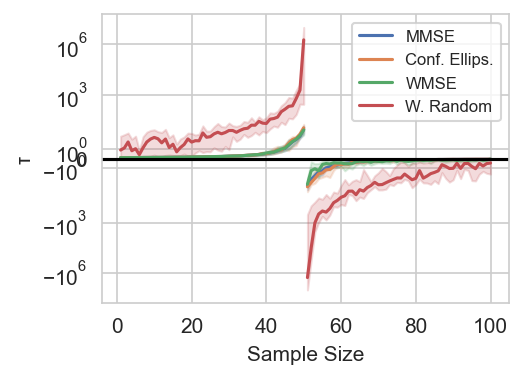
\includegraphics[width=\columnwidth]{figures/proj1/plots/LS_threshold/ER_0pt8_500_bandwidth_50_thresholds_LS.png}}
    \caption{Erdős–Rényi, 500 vertices} 
    \label{snr_ER}
    \end{subfigure}
    \hfill
    \begin{subfigure}{0.3\columnwidth}
    \resizebox{\width}{0.62\columnwidth}{
    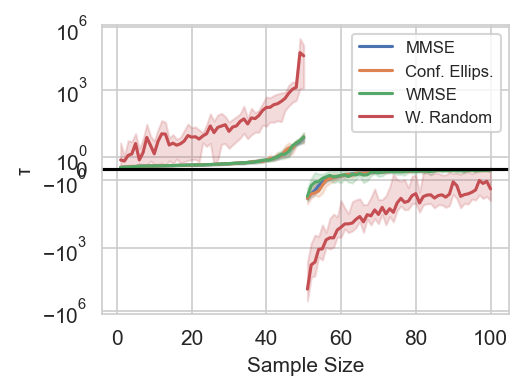
\includegraphics[width=\columnwidth]{figures/proj1/plots/LS_threshold/BA_3_500_bandwidth_50_thresholds_LS.png}}
    \caption{Barabási-Albert, 500 vertices}%
    \label{snr_BA}%
    \end{subfigure}
    \hfill%
    \begin{subfigure}{0.3\columnwidth}
    \resizebox{\width}{0.62\columnwidth}{
    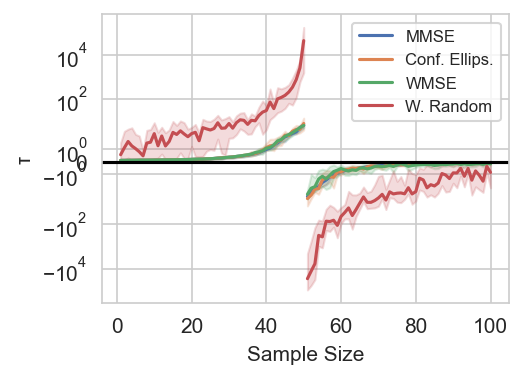
\includegraphics[width=\columnwidth]{figures/proj1/plots/LS_threshold/SBM_500_bandwidth_50_thresholds_LS.png}}
    \caption{SBM, 500 vertices}%
    \label{snr_SBM}%
    \end{subfigure}%
    \hfill
    \begin{subfigure}{0.3\columnwidth}
    \resizebox{\width}{0.62\columnwidth}{
    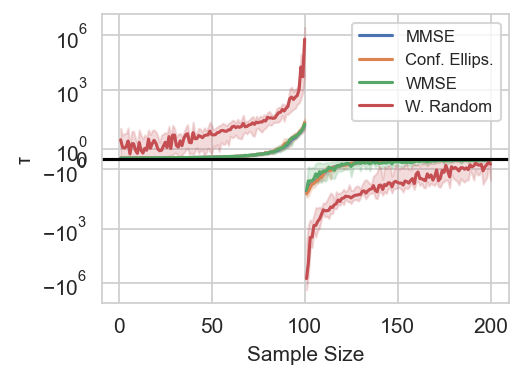
\includegraphics[width=\columnwidth]{figures/proj1/plots/LS_threshold/ER_0pt8_1000_bandwidth_100_thresholds_LS.png}}
    \caption{Erdős–Rényi, 1000 vertices} 
    \label{snr_ER_1000}
    \end{subfigure}
    \hfill
    \begin{subfigure}{0.3\columnwidth}
    \resizebox{\width}{0.62\columnwidth}{
    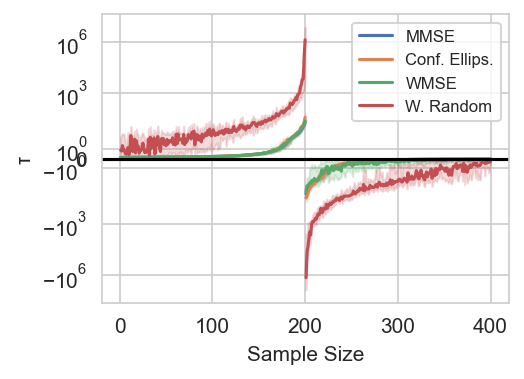
\includegraphics[width=\columnwidth]{figures/proj1/plots/LS_threshold/ER_0pt8_2000_bandwidth_200_thresholds_LS.png}}
    \caption{Erdős–Rényi, 2000 vertices}%
    \label{snr_ER_2000}%
    \end{subfigure}
    \hfill%
    \begin{subfigure}{0.3\columnwidth}
    \resizebox{\width}{0.62\columnwidth}{
    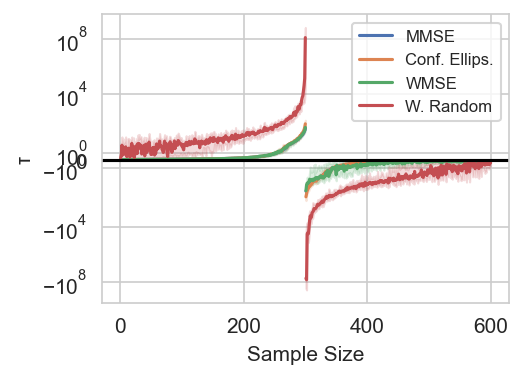
\includegraphics[width=\columnwidth]{figures/proj1/plots/LS_threshold/ER_0pt8_3000_bandwidth_300_thresholds_LS.png}}
    \caption{Erdős–Rényi, 3000 vertices}%
    \label{snr_ER_3000}%
    \end{subfigure}%
    \caption{$\tau(\set{S},v)$ for different random graph models and different $N$ under LS and full-band noise (bandwidth = $\frac{\# \text{ vertices}}{10}$)}
%\label{LS_SNR_Threshold_plots_big}
\label{LS_SNR_Threshold_plots_all}
\end{figure*}

%GLR_threshold_plots

\begin{figure*}%
    \centering
    \begin{subfigure}{0.3\columnwidth}
    \resizebox{\width}{0.62\columnwidth}{
    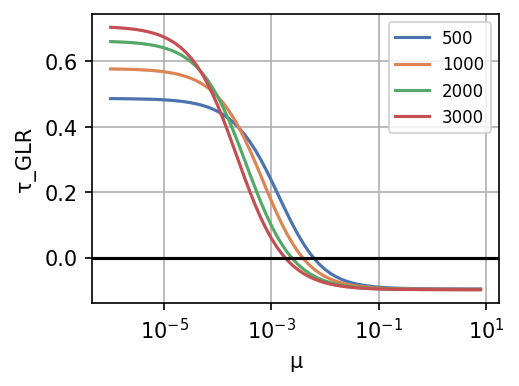
\includegraphics[width=\columnwidth]{figures/proj1/plots/GLR_threshold/ER_fb.png}}
    \caption{Erdős–Rényi ($\tau_{GLR}$)}
    \label{tau_GLR_er}
    \end{subfigure}
    \hfill
    \begin{subfigure}{0.3\columnwidth}
    \resizebox{\width}{0.62\columnwidth}{
    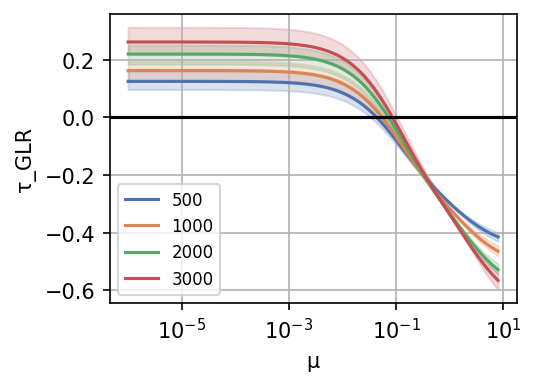
\includegraphics[width=\columnwidth]{figures/proj1/plots/GLR_threshold/BA_fb.png}}
    \caption{Barabási-Albert ($\tau_{GLR}$)}%
    \label{tau_GLR_BA}%
    \end{subfigure}
    \hfill%
    \begin{subfigure}{0.3\columnwidth}
    \resizebox{\width}{0.62\columnwidth}{
    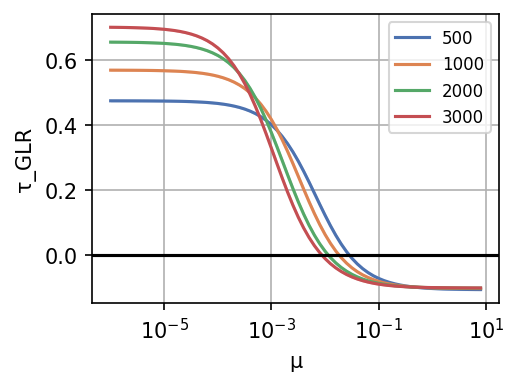
\includegraphics[width=\columnwidth]{figures/proj1/plots/GLR_threshold/SBM_fb.png}}
    \caption{SBM ($\tau_{GLR}$)}%
    \label{tau_GLR_SBM}%
    \end{subfigure}%
    \hfill
    \caption{$\tau_{GLR}$  for different random graph models (\#vertices = colour, bandwidth = $\frac{\text{\# vertices}}{10}$)}
\label{GLR_Threshold_plots}
\end{figure*}


%ER MSEs
\begin{figure*}%
    \centering
    \begin{subfigure}{0.3\columnwidth}
    \resizebox{\width}{0.62\columnwidth}{
    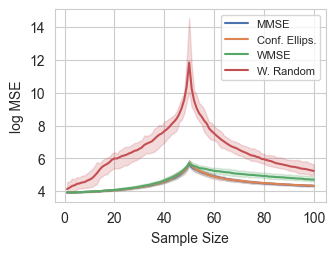
\includegraphics[width=\columnwidth]{figures/proj1/plots/LS_MSE/ER_0pt8_500_bandwidth_50_SNRdbs_-10.0_samps_100_MSE_LS.png}}
    \caption{Full-band noise, SNR = $10^{-1}$}
    \label{MSE_subfiga}
    \end{subfigure}\hfill
    \begin{subfigure}{0.3\columnwidth}
    \resizebox{\width}{0.62\columnwidth}{
    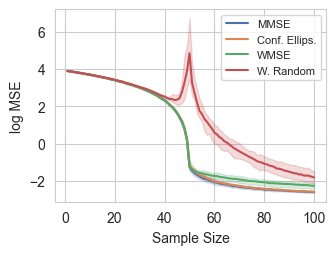
\includegraphics[width=\columnwidth]{figures/proj1/plots/LS_MSE/ER_0pt8_500_bandwidth_50_SNRdbs_20.0_samps_100_MSE_LS.png}}
    \caption{Full-band noise, SNR = $10^{2}$}%
    \label{MSE_subfigb}%
    \end{subfigure}\hfill%
    \begin{subfigure}{0.3\columnwidth}
    \resizebox{\width}{0.62\columnwidth}{
    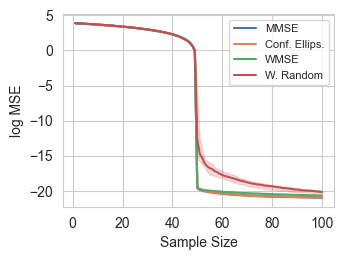
\includegraphics[width=\columnwidth]{figures/proj1/plots/LS_MSE/ER_0pt8_500_bandwidth_50_SNRdbs_100.0_samps_100_MSE_LS.png}}
    \caption{Full-band noise, SNR = $10^{10}$}%
    \label{MSE_subfigc}%
    \end{subfigure}%
    \caption{Average MSE under LS on ER Graphs (\#vertices=500, bandwidth = 50) }
\label{LS_ER_MSE_fig}
\end{figure*}



\begin{figure*}%
    \centering
    \begin{subfigure}{0.3\columnwidth}
    \resizebox{\width}{0.62\columnwidth}{
    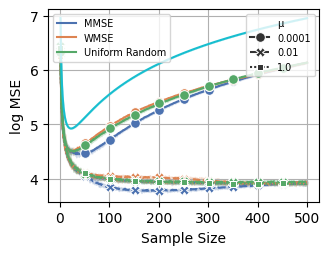
\includegraphics[width=\columnwidth]{figures/proj1/plots/GLR_MSE/ER_0pt8_500_bandwidth_50_SNRdbs_-10.0_samps_500_mus_0.0001_0.01_1_full_band.png}}
    \caption{Full-band noise, SNR = $10^{-1}$}
    \label{GLR_MSE_subfiga}
    \end{subfigure}\hfill
    \begin{subfigure}{0.3\columnwidth}
    \resizebox{\width}{0.62\columnwidth}{
    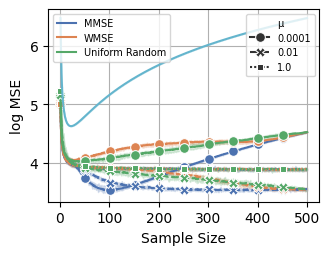
\includegraphics[width=\columnwidth]{figures/proj1/plots/GLR_MSE/ER_0pt8_500_bandwidth_50_SNRdbs_-3.01_samps_500_mus_0.0001_0.01_1_full_band.png}}
    \caption{Full-band noise, SNR = $\frac{1}{2}$}%
    \label{GLR_MSE_subfigb}%
    \end{subfigure}\hfill%
    \begin{subfigure}{0.3\columnwidth}
    \resizebox{\width}{0.62\columnwidth}{
    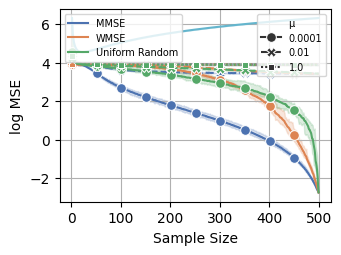
\includegraphics[width=\columnwidth]{figures/proj1/plots/GLR_MSE/ER_0pt8_500_bandwidth_50_SNRdbs_100.0_samps_500_mus_0.0001_0.01_1_full_band.png}}
    \caption{Full-band noise, SNR = $10^{10}$}%
    \label{GLR_MSE_subfigc}%
    \end{subfigure}%
    \caption{Average MSE under GLR on ER Graphs (\#vertices=500, bandwidth = 50), line without markers is an upper bound}
\label{GLR_ER_MSE_fig}
%\label{bandlimited_GLR_ER_MSE_fig}
\end{figure*}

%%% REAL DATASET experiments

\begin{figure}
    \centering
    \begin{subfigure}{0.3\columnwidth}
    %\resizebox{\width}{0.75\columnwidth}
    \resizebox{\width}{0.62\columnwidth}
    {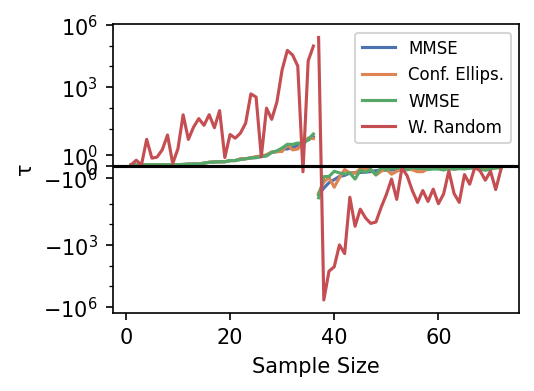
\includegraphics[width=\columnwidth]{figures/proj1/plots/LS_threshold_real/fmri_subsample_500_367_bandwidth_36_thresholds_LS.png}}
    \caption{FMRI} 
    \label{snr_FMRI}
    \end{subfigure}
    \begin{subfigure}{0.3\columnwidth}
    \resizebox{\width}{0.62\columnwidth}{
    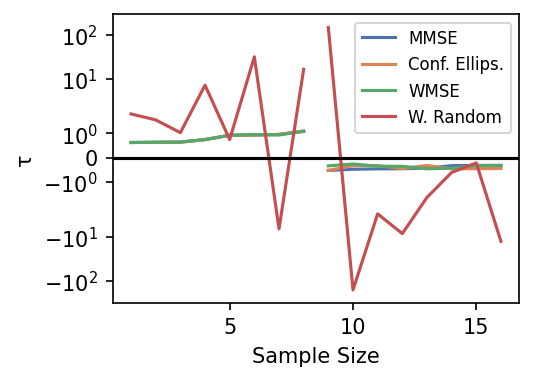
\includegraphics[width=\columnwidth]{figures/proj1/plots/LS_threshold_real/weather_45_bandwidth_8_thresholds_LS.png}}
    \caption{Weather}%
    \label{snr_Weather}%
    \end{subfigure}
    \caption{$\tau(\set{S},v)$ for real world datasets under LS and full-band noise}
\label{LS_SNR_Threshold_plots_all_real}
\end{figure}

\begin{figure}%
    \centering
    \begin{subfigure}{0.3\columnwidth}
    \resizebox{\width}{0.62\columnwidth}{
    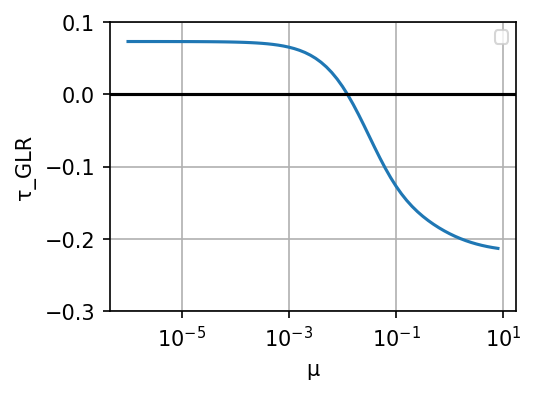
\includegraphics[width=\columnwidth]{figures/proj1/plots/GLR_threshold_real/fmri_subsample_500_GLR_threshold_fb.png}}
    \caption{FMRI}
    \label{tau_GLR_fmri}
    \end{subfigure}
    \begin{subfigure}{0.3\columnwidth}
    \resizebox{\width}{0.62\columnwidth}{
    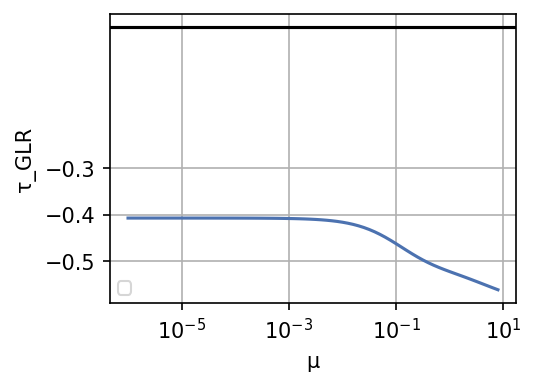
\includegraphics[width=\columnwidth]{figures/proj1/plots/GLR_threshold_real/weather_GLR_threshold_fb.png}}
    \caption{Weather}%
    \label{tau_GLR_weather}%
    \end{subfigure}
    \caption{$\tau_{GLR}$ for real world datasets}
\label{GLR_Threshold_plots_real}
\end{figure}


\begin{figure*}%
    \centering
    \begin{subfigure}{0.3\columnwidth}
    \resizebox{\width}{0.62\columnwidth}{
    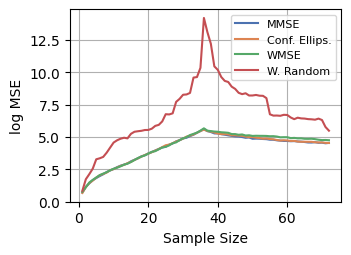
\includegraphics[width=\columnwidth]{figures/proj1/plots/LS_MSE_real/fmri_subsample_500_367_bandwidth_36_SNRdbs_-10.0_samps_72_fb_blsig_MSE_LS.png}}
    \caption{FMRI, SNR = $10^{-1}$}
    \label{fmri_MSE_subfiga}
    \end{subfigure}\hfill
    \begin{subfigure}{0.3\columnwidth}
    \resizebox{\width}{0.62\columnwidth}{
    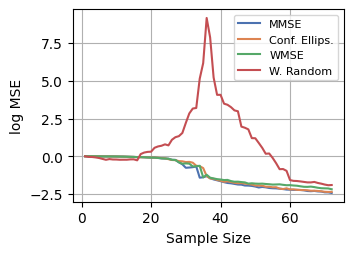
\includegraphics[width=\columnwidth]{figures/proj1/plots/LS_MSE_real/fmri_subsample_500_367_bandwidth_36_SNRdbs_20.0_samps_72_fb_blsig_MSE_LS.png}}
    \caption{FMRI, SNR = $10^{2}$}%
    \label{fmri_MSE_subfigb}%
    \end{subfigure}\hfill%
    \begin{subfigure}{0.3\columnwidth}
    \resizebox{\width}{0.62\columnwidth}{
    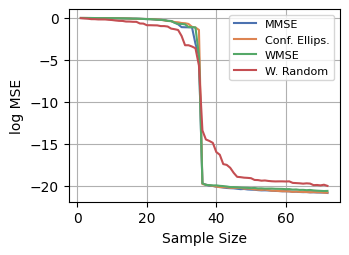
\includegraphics[width=\columnwidth]{figures/proj1/plots/LS_MSE_real/fmri_subsample_500_367_bandwidth_36_SNRdbs_100.0_samps_72_fb_blsig_MSE_LS.png}}
    \caption{FMRI, SNR = $10^{10}$}%
    \label{fmri_MSE_subfigc}%
    \end{subfigure}%
    \hfill
    \begin{subfigure}{0.3\columnwidth}
    \resizebox{\width}{0.62\columnwidth}{
    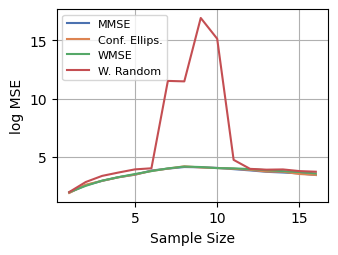
\includegraphics[width=\columnwidth]{figures/proj1/plots/LS_MSE_real/weather_45_bandwidth_8_SNRdbs_-10.0_samps_16_fb_blsig_MSE_LS.png}}
    \caption{Weather, SNR = $10^{-1}$}
    \label{weather_MSE_subfiga}
    \end{subfigure}\hfill
    \begin{subfigure}{0.3\columnwidth}
    \resizebox{\width}{0.62\columnwidth}{
    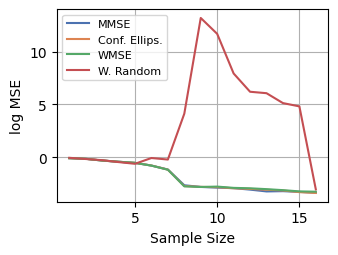
\includegraphics[width=\columnwidth]{figures/proj1/plots/LS_MSE_real/weather_45_bandwidth_8_SNRdbs_20.0_samps_16_fb_blsig_MSE_LS.png}}
    \caption{Weather, SNR = $1$}%
    \label{weather_MSE_subfigb}%
    \end{subfigure}\hfill%
    \begin{subfigure}{0.3\columnwidth}
    \resizebox{\width}{0.62\columnwidth}{
    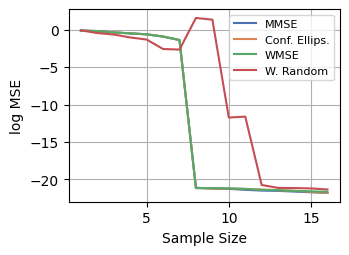
\includegraphics[width=\columnwidth]{figures/proj1/plots/LS_MSE_real/weather_45_bandwidth_8_SNRdbs_100.0_samps_16_fb_blsig_MSE_LS.png}}
    \caption{Weather, SNR = $10^{10}$}%
    \label{weather_MSE_subfigc}%
    \end{subfigure}%
    \caption{Average MSE under LS on real world datasets and full-band noise }
\label{LS_real_MSE_fig}
\end{figure*}

\begin{figure*}%
    \centering
    \begin{subfigure}{0.3\columnwidth}
    \resizebox{\width}{0.62\columnwidth}{
    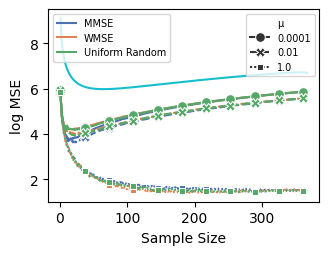
\includegraphics[width=\columnwidth]{figures/proj1/plots/GLR_MSE_real/fmri_subsample_500_367_bandwidth_36_SNRdbs_-10.0_samps_367_mus_0.0001_0.01_1_full_band_MSE_GLR.png}}
    \caption{FMRI, SNR = $10^{-1}$}
    \label{fmri_GLR_MSE_subfiga}
    \end{subfigure}\hfill
    \begin{subfigure}{0.3\columnwidth}
    \resizebox{\width}{0.62\columnwidth}{
    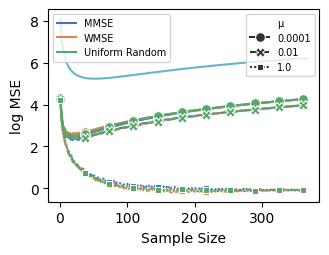
\includegraphics[width=\columnwidth]{figures/proj1/plots/GLR_MSE_real/fmri_subsample_500_367_bandwidth_36_SNRdbs_-3.010299956639812_samps_367_mus_0.0001_0.01_1_full_band_MSE_GLR.png}}
    \caption{FMRI, SNR = $\frac{1}{2}$}%
    \label{fmri_GLR_MSE_subfigb}%
    \end{subfigure}\hfill%
    \begin{subfigure}{0.3\columnwidth}
    \resizebox{\width}{0.62\columnwidth}{
    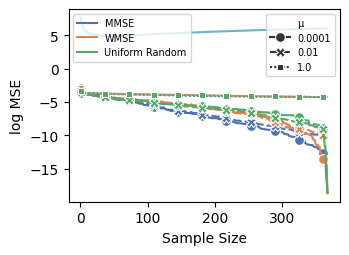
\includegraphics[width=\columnwidth]{figures/proj1/plots/GLR_MSE_real/fmri_subsample_500_367_bandwidth_36_SNRdbs_100.0_samps_367_mus_0.0001_0.01_1_full_band_MSE_GLR.png}}
    \caption{FMRI, SNR = $10^{10}$}%
    \label{fmri_GLR_MSE_subfigc}%
    \end{subfigure}%
    \hfill
    \begin{subfigure}{0.3\columnwidth}
    \resizebox{\width}{0.62\columnwidth}{
    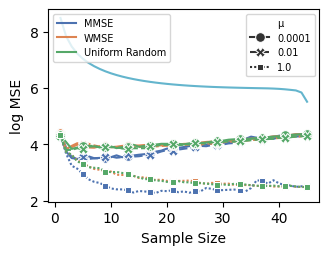
\includegraphics[width=\columnwidth]{figures/proj1/plots/GLR_MSE_real/weather_45_bandwidth_8_SNRdbs_-10.0_samps_45_mus_0.0001_0.01_1_full_band_MSE_GLR.png}}
    \caption{Weather, SNR = $10^{-2}$}
    \label{weather_GLR_MSE_subfiga}
    \end{subfigure}\hfill
    \begin{subfigure}{0.3\columnwidth}
    \resizebox{\width}{0.62\columnwidth}{
    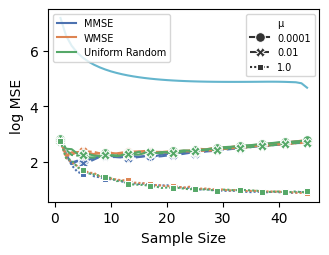
\includegraphics[width=\columnwidth]{figures/proj1/plots/GLR_MSE_real/weather_45_bandwidth_8_SNRdbs_-3.010299956639812_samps_45_mus_0.0001_0.01_1_full_band_MSE_GLR.png}}
    \caption{Weather, SNR = $\frac{1}{2}$}%
    \label{weather_GLR_MSE_subfigb}%
    \end{subfigure}\hfill%
    \begin{subfigure}{0.3\columnwidth}
    \resizebox{\width}{0.62\columnwidth}{
    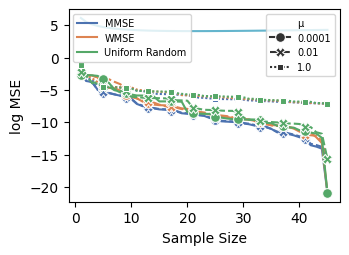
\includegraphics[width=\columnwidth]{figures/proj1/plots/GLR_MSE_real/weather_45_bandwidth_8_SNRdbs_100.0_samps_45_mus_0.0001_0.01_1_full_band_MSE_GLR.png}}
    \caption{Weather, SNR = $10^{10}$}%
    \label{weather_GLR_MSE_subfigc}%
    \end{subfigure}%
    \caption{Average MSE under GLR on real world datasets, line without markers is an upper bound}
\label{GLR_real_MSE_fig}
%\label{bandlimited_GLR_ER_MSE_fig}
\end{figure*}
\fi

Our theoretical results show how the relationship between sample size and MSE changes with the level of noise, focusing on how reducing sample size will reduce MSE if the SNR is below a threshold. In this section, we demonstrate  the applicability and validity of these results via empirical experiments. 

%Note that we always consider SNR in ratio form --- as $10^{x}$ rather than $\frac{x}{10} dB$ --- which is always positive. For the SNR to be below a given threshold (and so for us to show reducing sample size will decrease MSE) the threshold must be positive.

We first demonstrate the applicability of our results with plots of the thresholds $\tau(\set{S},v)$, $\tau_{GLR}$ and $\tau_{GLR\_bl}$ against sample size (Figs. \ref{LS_SNR_Threshold_plots_all} and \ref{GLR_Threshold_plots}). These plots show concrete SNR values for the thresholds, giving a practical understanding of how high noise levels need to be for reducing sample size to reduce MSE for different random graph models and parameters. Additionally, we empirically tabulate the probabilities that graphs from each model  satisfy the conditions of our theorems (Table \ref{tbl:empirical_probabilities_conditions}), allowing the reader to evaluate the impact of our theorems across different applications. We then demonstrate the validity of our results by plotting $\textrm{MSE}_{\set{S}}$ against sample size (Figs. \ref{LS_ER_MSE_fig} and  \ref{GLR_ER_MSE_fig}) at SNRs below, near and above the derived thresholds, showing that the behaviour of $\textrm{MSE}_{\set{S}}$ follows our theoretical results. \bs{We finally present similar results on real-world datasets, validating the applicability of our results to real world datasets.}

\subsection{Experimental Setup}
We now present the setup of the experiments. All results are presented with 90\% confidence intervals and all experiments use the combinatorial Laplacian $\matr{L}$ and its eigenbasis.
\subsubsection{\bs{Synthetic} Graph Generation}
We consider each of the following unweighted random graph models:
\begin{itemize}
    \item Erdős–Rényi (ER) with edge probability $p=0.8$ (experiments with other values of $p$ show similar results)
    \item Barabási-Albert (BA) with a preferential attachment to 3 vertices at each step of its construction
    \item Stochastic Blockmodel (SBM) with intra- and inter-cluster edge probabilities of $0.7 \text{ and }0.1$ respectively
    %\item Ring (Ring).
\end{itemize}
We consider 10 instantiations of each model for plots, and 1000 instantiations of each model to assess the probability the graph invariant conditions in our Theorems are met.

We present threshold plots for graphs with 500, 1000, 2000 and 3000 vertices. We only present MSE plots for graphs with 500 vertices  {\color{black}  (like \cite[Fig 8]{bai2020fast})} as they are intended as an accompaniment to our threshold plots and theorems to demonstrate their validity, and a single graph size suffices. 

\subsubsection{\xd{Synthetic} Signal Generation}
We set the bandwidth  $k = \lfloor \frac{N}{10} \rfloor$, as per \cite{bai2020fast}.  We consider the following SNRs:

\begin{itemize}
    \item{\makebox[8em][l]{Full-band noise:}  $10^{-1}, 10^{2}, 10^{10}$ (i.e. $-10dB, 20dB, 100dB$)}
    \item{\makebox[8em][l]{Bandlimited noise:}  $10^{-1}, 1, 10^{10}$ (i.e. $-10dB, 0dB, 100dB$)}
\end{itemize}
These SNRs are chosen to demonstrate that there are three regimes for MSE with distinctive properties---the high noise regime, the transitionary regime and the approximately noiseless regime---and that $\tau$ captures when the regimes change. Suitable values of SNRs to demonstrate this vary between reconstruction methods and noise types, hence our choices.
%Note that we always consider SNR in ratio form---as $10^{x}$ rather than $\frac{x}{10} dB$---which is always positive. For the SNR to be below a given threshold (and so for us to show reducing sample size will decrease MSE) the threshold must be positive.

To test the MSE in reconstructing signals from samples \bs{on random graph models}, we generate 200 signals by sampling $\vect{y} = \vect{x}_{raw} + \sigma \cdot \epsilon_{raw}$ where:
\begin{enumerate}
    \item $\vect{x}_{raw} \sim \mathcal{N}(\vect{0}, \matr{\Pi}_{bl(\set{K})})$ 
    \item[2a)] If full-band noise, $\vect{\epsilon}_{raw} \sim \mathcal{N}(\vect{0}, \matr{I}_{N})$, $\sigma = \sqrt{\frac{k}{{N \cdot\text{SNR}}}}$
    \item[2b)]  If bandlimited noise, $\vect{\epsilon}_{raw} \sim \mathcal{N}(\vect{0}, \projbl )$, $\sigma = \frac{1}{\sqrt{\text{SNR}}}$ 
    %\item Normalise $\vect{x}_{raw}$ and $\vect{\epsilon}_{raw}$ to have norm 1
    %\item Normalise: $\vect{x} = \frac{\vect{x}_{raw}}{||\vect{x}_{raw}||_{2}}$ and $\vect{\epsilon} = \frac{\vect{\epsilon}_{raw}}{ ||\vect{\epsilon}_{raw}||_{2}}$
    %\item[3)] Return $\vect{y} = \vect{x} + \frac{\vect{\epsilon}}{\sqrt{\text{SNR}}}$
    %\item[3)] Return $\vect{y} = \vect{x} + \sigma \cdot \epsilon$
\end{enumerate}
%For the cases of bandlimited noise, in step (1) we generate $\vect{\epsilon}_{raw} \sim \mathcal{N}(\vect{0}, \projbl )$ instead.

\subsubsection{Real World Datasets}
\bs{
We also consider two real world datasets as in \cite{zhi2023gaussian}. The first is an FMRI dataset, where the original graph consists of 4465 nodes corresponding to voxels of the cerebellum, with 292 Blood-Oxygen-Level-Dependent (BOLD) signals derived from FMRI. We sample a connected subgraph of 367 nodes via Neighbourhood Sampling \cite{hamilton2017inductive}. The second is a Weather dataset, where a $10$-nearest neighbours graph of 45 cities in Sweden is constructed, with 95 signals derived from the temperature. See \cite{venkitaraman2020gaussian, behjat2016signal, zhi2023gaussian} for details on graph construction and signal generation in both cases. 
We generate $\vect{x}$ by $k$-bandlimiting the original signals, where For FMRI we set $k=36$ and for Weather dataset we set $k=8$. We otherwise follow the above methodology in Synthetic Signal Generation for generating signals with full-band noise.
}


\subsubsection{Sample-Set Selection}
%The literature provides several approximations to make vertex sample-set selection efficient; for example, approximating the projection matrix $\projbl$ \cite{wang2018optimal} (subsets of which are used to compute optimality criteria) with a polynomial in $\matr{L}$, and approximating optimality criteria for easier computation \cite{bai2020fast}. 

We generate sample sets greedily using exact analytic forms and by exactly computing $\matr{\Pi}_{bl(\set{K})}$.
\begin{itemize}
    \item[LS:] We use (\ref{eq:A-optimality})-(\ref{eq:E-optimality}) to exactly compute the MMSE {\color{black}\cite{wang2018optimal,wang2019low, mfn}}, Confidence Ellipsoid {\color{black}\cite{jayawant2021doptimal, tremblay2017determinantal,mfn}} and WMSE criteria {\color{black} \cite{bai2020fast}}, which are deterministic and guaranteed to be noiseless-optimal.  We also look at Weighted Random sampling \cite{puy2018random}, which is neither deterministic nor guaranteed to be noiseless-optimal.
\end{itemize}
Note that sampling schemes in the literature tend to differ from ours mainly in that they approximate our setup for computational efficiency reasons; e.g. approximating the projection matrix $\projbl$ with a polynomial in $\matr{L}$ \cite{wang2018optimal}, and approximating optimality criteria \cite{bai2020fast}. As these differences are for efficiency reasons, we do not expect them to matter in our experiments.

\subsubsection{Parameters of Reconstruction Methods} We consider LS with the previously stated bandwidth.

\subsection{Experimental Results --- Synthetic Graphs}

\begin{figure*}
    \centering
    \begin{subfigure}{0.3\columnwidth}
    %\resizebox{\width}{0.75\columnwidth}
    \resizebox{\width}{0.62\columnwidth}
    {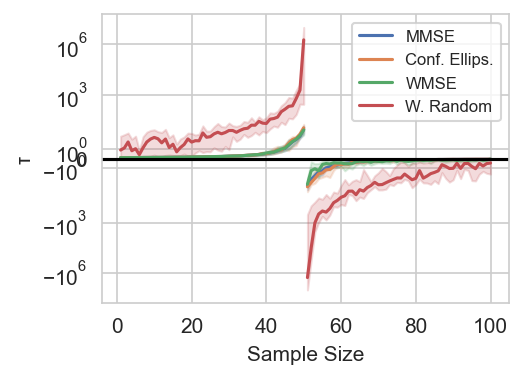
\includegraphics[width=\columnwidth]{figures/proj1/plots/LS_threshold/ER_0pt8_500_bandwidth_50_thresholds_LS.png}}
    \caption{Erdős–Rényi, 500 vertices} 
    \label{snr_ER}
    \end{subfigure}
    \hfill
    \begin{subfigure}{0.3\columnwidth}
    \resizebox{\width}{0.62\columnwidth}{
    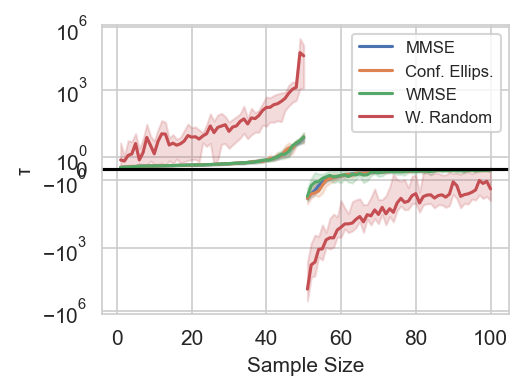
\includegraphics[width=\columnwidth]{figures/proj1/plots/LS_threshold/BA_3_500_bandwidth_50_thresholds_LS.png}}
    \caption{Barabási-Albert, 500 vertices}%
    \label{snr_BA}%
    \end{subfigure}
    \hfill%
    \begin{subfigure}{0.3\columnwidth}
    \resizebox{\width}{0.62\columnwidth}{
    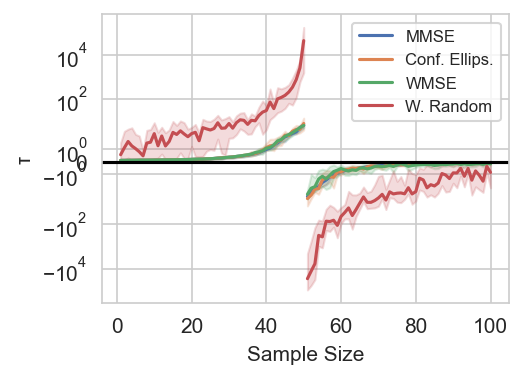
\includegraphics[width=\columnwidth]{figures/proj1/plots/LS_threshold/SBM_500_bandwidth_50_thresholds_LS.png}}
    \caption{SBM, 500 vertices}%
    \label{snr_SBM}%
    \end{subfigure}%
    \hfill
    \begin{subfigure}{0.3\columnwidth}
    \resizebox{\width}{0.62\columnwidth}{
    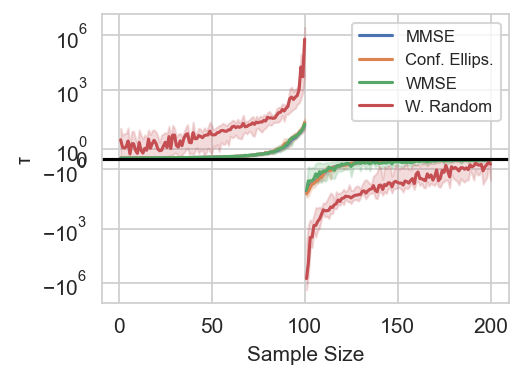
\includegraphics[width=\columnwidth]{figures/proj1/plots/LS_threshold/ER_0pt8_1000_bandwidth_100_thresholds_LS.png}}
    \caption{Erdős–Rényi, 1000 vertices} 
    \label{snr_ER_1000}
    \end{subfigure}
    \hfill
    \begin{subfigure}{0.3\columnwidth}
    \resizebox{\width}{0.62\columnwidth}{
    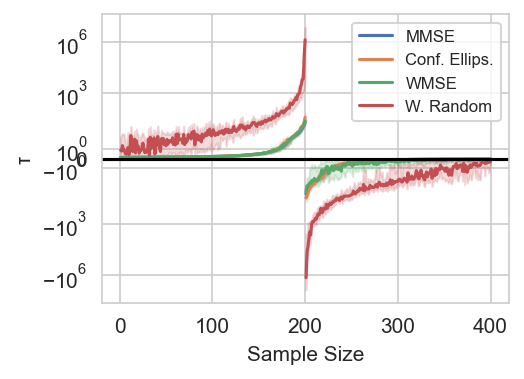
\includegraphics[width=\columnwidth]{figures/proj1/plots/LS_threshold/ER_0pt8_2000_bandwidth_200_thresholds_LS.png}}
    \caption{Erdős–Rényi, 2000 vertices}%
    \label{snr_ER_2000}%
    \end{subfigure}
    \hfill%
    \begin{subfigure}{0.3\columnwidth}
    \resizebox{\width}{0.62\columnwidth}{
    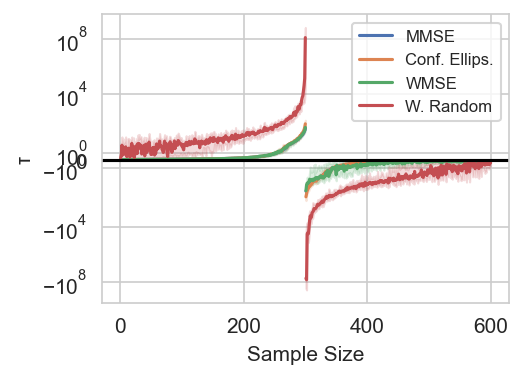
\includegraphics[width=\columnwidth]{figures/proj1/plots/LS_threshold/ER_0pt8_3000_bandwidth_300_thresholds_LS.png}}
    \caption{Erdős–Rényi, 3000 vertices}%
    \label{snr_ER_3000}%
    \end{subfigure}%
    \caption{$\tau(\set{S},v)$ for different random graph models and different $N$ under LS and full-band noise (bandwidth = $\frac{\# \text{ vertices}}{10}$)}
%\label{LS_SNR_Threshold_plots_big}
\label{LS_SNR_Threshold_plots_all}
\end{figure*}

%GLR_threshold_plots

\begin{figure*}%
    \centering
    \begin{subfigure}{0.3\columnwidth}
    \resizebox{\width}{0.62\columnwidth}{
    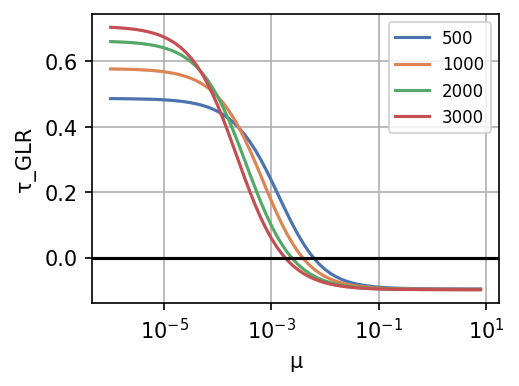
\includegraphics[width=\columnwidth]{figures/proj1/plots/GLR_threshold/ER_fb.png}}
    \caption{Erdős–Rényi ($\tau_{GLR}$)}
    \label{tau_GLR_er}
    \end{subfigure}
    \hfill
    \begin{subfigure}{0.3\columnwidth}
    \resizebox{\width}{0.62\columnwidth}{
    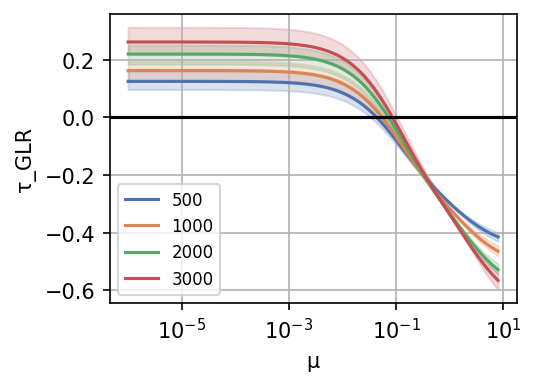
\includegraphics[width=\columnwidth]{figures/proj1/plots/GLR_threshold/BA_fb.png}}
    \caption{Barabási-Albert($\tau_{GLR}$)}%
    \label{tau_GLR_BA}%
    \end{subfigure}
    \hfill%
    \begin{subfigure}{0.3\columnwidth}
    \resizebox{\width}{0.62\columnwidth}{
    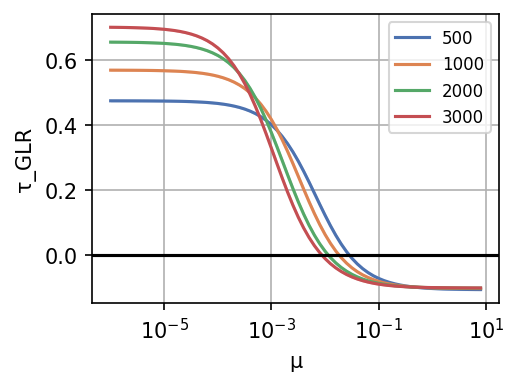
\includegraphics[width=\columnwidth]{figures/proj1/plots/GLR_threshold/SBM_fb.png}}
    \caption{SBM ($\tau_{GLR}$)}%
    \label{tau_GLR_SBM}%
    \end{subfigure}%
    \hfill
    \caption{$\tau_{GLR}$  for different random graph models (\#vertices = colour, bandwidth = $\frac{\text{\# vertices}}{10}$)}
\label{GLR_Threshold_plots}
\end{figure*}


%ER MSEs
\begin{figure*}%
    \centering
    \begin{subfigure}{0.3\columnwidth}
    \resizebox{\width}{0.62\columnwidth}{
    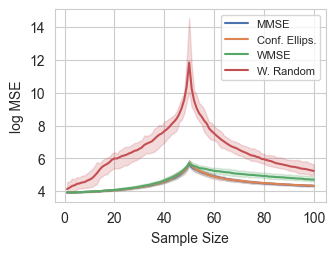
\includegraphics[width=\columnwidth]{figures/proj1/plots/LS_MSE/ER_0pt8_500_bandwidth_50_SNRdbs_-10.0_samps_100_MSE_LS.png}}
    \caption{Full-band noise, SNR = $10^{-1}$}
    \label{MSE_subfiga}
    \end{subfigure}\hfill
    \begin{subfigure}{0.3\columnwidth}
    \resizebox{\width}{0.62\columnwidth}{
    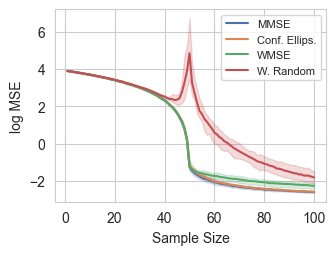
\includegraphics[width=\columnwidth]{figures/proj1/plots/LS_MSE/ER_0pt8_500_bandwidth_50_SNRdbs_20.0_samps_100_MSE_LS.png}}
    \caption{Full-band noise, SNR = $10^{2}$}%
    \label{MSE_subfigb}%
    \end{subfigure}\hfill%
    \begin{subfigure}{0.3\columnwidth}
    \resizebox{\width}{0.62\columnwidth}{
    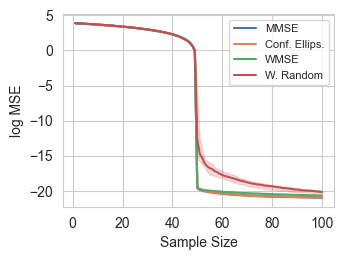
\includegraphics[width=\columnwidth]{figures/proj1/plots/LS_MSE/ER_0pt8_500_bandwidth_50_SNRdbs_100.0_samps_100_MSE_LS.png}}
    \caption{Full-band noise, SNR = $10^{10}$}%
    \label{MSE_subfigc}%
    \end{subfigure}%
    \caption{Average MSE under LS on ER Graphs (\#vertices=500, bandwidth = 50) }
\label{LS_ER_MSE_fig}
\end{figure*}





For full-band noise, we present threshold plots for all graphs and MSE plots for ER graphs in the main body of the paper. MSE plots for BA and SBM graphs are presented in Appendix \ref{plot_appendix}. For bandlimited noise, we present threshold plots, MSE plots and discussion of how the experimental and theoretical results correspond in Appendix \ref{app:Experiments_Bandlimited}.
{\color{black} We also present Table \ref{tbl:theory_experiment_correspondence} showing how our plots correspond to our theoretical results, which also corresponds to the summary of theoretical results in Table \ref{tbl:general_theory}.}

\iffalse
\begin{table}[h]
{\color{black}
\caption{Correspondence of Theory and Empirical Results}
\centering
\begin{tabularx}{(\textwidth)}{|X|p{2.6cm}|p{2.5cm}|p{2.6cm}|p{2.6cm}|}%{|@{\hspace{0.1cm}}p{2.6cm}|p{2.6cm}|p{2.6cm}|p{2.6cm}|X|}
\hline
\multirow{2}{*}{} & \multicolumn{2}{c|}{\textbf{LS}} & \multicolumn{2}{c|}{\textbf{GLR}} \\
\cline{2-5}
 & Full-band & Bandlimited & Full-band & Bandlimited \\
\hline
\textbf{Character- isation} & 
\makecell{Corr \ref{main_ls} \\
(Figs. \ref{snr_ER}-\ref{snr_SBM}\\
\& \ref{MSE_subfiga}-\ref{MSE_subfigc})} & 
\makecell{Corr \ref{corr:LS_bandlimited_noise_big_variance} \\ (Figs. \ref{bandlimited_MSE_subfiga}-\\ \ref{bandlimited_MSE_subfigc})} & 
\multicolumn{2}{c|}{\makecell{Corr \ref{corr:main_GLR_iff} \\ (Figs. \ref{GLR_MSE_subfiga}-\ref{GLR_MSE_subfigc})}
} \\
\hline
\textbf{Existence} & 
\makecell{Thm \ref{thm:noiseless_optimality_means_noise_sensitivity} \\ (Figs. \ref{snr_ER}-\ref{snr_SBM}\\
\& \ref{MSE_subfiga}-\ref{MSE_subfigc})} & 
\makecell{Corr \ref{corr:LS_bandlimited_noise_sample_only_k} \\ (Figs. \ref{bandlimited_MSE_subfiga}- \\ \ref{bandlimited_MSE_subfigc})} & 
\makecell{Thm \ref{thm:main_GLR_exist} \\
 (Figs. \ref{tau_GLR_er}-\ref{tau_GLR_SBM} \\ \& \ref{GLR_MSE_subfiga}-\ref{GLR_MSE_subfigc}\\
 \& Table \ref{tbl:empirical_probabilities_conditions})
} & 
\makecell{Thm \ref{thm:main_GLR_bl} \\
(Figs. \ref{tau_GLR_bl_er}-\ref{tau_GLR_bl_SBM} \\ \& \ref{bandlimited_GLR_MSE_subfiga}-\ref{bandlimited_GLR_MSE_subfigc} \\
\& Table \ref{tbl:empirical_probabilities_conditions_bl})
} \\
\hline
\textbf{Asymptotics} & 
\makecell{Rmk \ref{rmk:LS_big_N} \\ (Figs. \ref{snr_ER_1000}-\ref{snr_ER_3000})} & 
\makecell{\\ Rmk \ref{rmk:LS_big_N_bl}} & 
\makecell{Propn \ref{propn:GLR_big_N} \\ (Figs. \ref{tau_GLR_er}-\ref{tau_GLR_SBM})} & 
\makecell{Propn \ref{propn:GLR_big_N_bl} \\ (Figs. \ref{tau_GLR_bl_er}-\ref{tau_GLR_bl_SBM})} \\
\hline
\end{tabularx}
\label{tbl:theory_experiment_correspondence}
}
\end{table}
\fi

% Table 1: LS columns only
\begin{table}[h]
\caption{Correspondence of Theory and Empirical Results - LS}
\centering
\begin{tabularx}{\textwidth}{l >{\centering\arraybackslash}p{15em} >{\centering\arraybackslash}X}
\toprule
& \multicolumn{2}{c}{\textbf{LS}} \\
\cmidrule(lr){2-3}
 & Full-band Noise & Bandlimited Noise \\
\midrule
\textbf{Characterisation} & 
\makecell[c]{Corr \ref{main_ls} \\
(Figs. \ref{snr_ER}-\ref{snr_SBM} 
\& \ref{MSE_subfiga}-\ref{MSE_subfigc})} & 
\makecell[c]{Corr \ref{corr:LS_bandlimited_noise_big_variance} \\ (Figs. \ref{bandlimited_MSE_subfiga}- \ref{bandlimited_MSE_subfigc})} \\
\midrule
\textbf{Existence} & 
\makecell[c]{Thm \ref{thm:noiseless_optimality_means_noise_sensitivity} \\ (Figs. \ref{snr_ER}-\ref{snr_SBM}
\& \ref{MSE_subfiga}-\ref{MSE_subfigc})} & 
\makecell[c]{Corr \ref{corr:LS_bandlimited_noise_sample_only_k} \\ (Figs. \ref{bandlimited_MSE_subfiga}- \ref{bandlimited_MSE_subfigc})} \\
\midrule
\textbf{Asymptotics} & 
\makecell[c]{Rmk \ref{rmk:LS_big_N} \\ (Figs. \ref{snr_ER_1000}-\ref{snr_ER_3000})} & 
\makecell[c]{Rmk \ref{rmk:LS_big_N_bl}\\} \\
\bottomrule
\end{tabularx}
\label{tbl:theory_experiment_correspondence_LS}
\end{table}



%\subsubsection{\texorpdfstring{$\tau$ and $\tau_{GLR}$ plots}{\texttau and \texttau\_GLR plots}}
\subsubsection{$\tau$ plots (LS)}

%Our threshold plots demonstrate the applicability of our theorems. We remember that SNR is in ratio form (not in $dB$) and so always positive by definition. We overlay a black line at $\tau = 0$ to emphasise how when $\tau > 0$ and $0 < \textrm{SNR} < \tau$, we have proven that reducing sample size can reduce MSE. 

%As the thresholds are bounds on the ratio form of SNR (not in $dB$), we overlay a black line at 0. This is meaningful because our theorems only say 
%Our threshold plots demonstrate the applicability of our theorems. Our threshold plots are bounds on the ratio form of SNR (not in $dB$), so the transition between negative and positive is important; therefore, we overlay a black line at 0.
%\,\\
%\emph{[LS]:} 
Figs. \ref{LS_SNR_Threshold_plots_all}  shows $\tau(\set{S},v)$ as sample size varies for sequential sampling methods under LS, where $v$ is the latest node added to $\set{S}$. 
 % We interpret the subfigures of Fig. \ref{LS_SNR_Threshold_plots}:
 % \begin{itemize}
     % \item[(a)] 
     For ER graphs, for sample size smaller than the bandwidth, $\tau(\set{S},v) > 0$ and beyond that $\tau(\set{S},v) \leq 0$. The maximum of $\tau(\set{S},v)$ observed is approximately $10^{6}$ ($60dB$) for weighted random sampling, and approximately 10 ($10dB$) for the deterministic sampling methods. The confidence intervals for weighted random sampling is much wider than for the deterministic sampling methods.
     Next, we observe the same phenomenon as with ER for BA and SBM graphs, with maxima of approximately $10^5$ ($50dB$) for weighted random sampling and maxima of approximately 10 ($10dB$) for the deterministic sampling methods.
% \end{itemize}
Finally, Figs. \ref{snr_ER_1000}-\ref{snr_ER_3000} show the same phenomenon as Fig. \ref{snr_ER} happens for ER graphs at sizes of 1000, 2000 and 3000 vertices.

 We now correlate our experiments and our theoretical results. As Corollary \ref{main_ls} is necessary and sufficient, the sign of $\tau(\set{S},v)$ tells us exactly when removing a vertex improves $\set{S}$. Therefore $\tau$ being negative is an informative statement, telling us that $\set{S} \backslash \{v\}$ is \emph{never} better than $\set{S}$. Concretely, if SNR is below the maximum $\tau(\set{S},v)$ observed, then when sample size equals bandwidth we can reduce sample size to reduce MSE.

 Theorem \ref{thm:noiseless_optimality_means_noise_sensitivity} proves that noiseless-optimal methods (MMSE, Confidence Ellipsoid and WMSE in our experiments) will have $\tau(\set{S},v) > 0$ for sample sizes smaller than the bandwidth, and then $\tau(\set{S},v) \leq 0$ afterwards, and Fig. \ref{LS_SNR_Threshold_plots_all}  validates this. Note that even though this pattern holds for Weighted Random Sampling in our experiments, Theorem \ref{thm:noiseless_optimality_means_noise_sensitivity} does not guarantee it always holds for Weighted Random Sampling.

 While we prove that $\tau(\set{S},v) \not\to 0$ as $N \to \infty$, we conjecture the stronger claim that at a sample size equal to bandwidth, $\tau(\set{S},v)$ might actually increase with graph size, which is supported (but not proven) by Figs. \ref{snr_ER_1000}-\ref{snr_ER_3000}.
 %We need $\textrm{SNR} > 10^{6}$ ($60dB$) for removing samples to not decrease MSE. %Comparing to the threshold plots for smaller $N$ (see Appendix \ref{plot_appendix}, Fig. \ref{fig:LS_SNR_Threshold_plots_small}) to Fig. \ref{LS_SNR_Threshold_plots} suggests that the thresholds get larger with $N$ --- a wider range of SNRs exhibit the phenomenon of reducing sample size reducing MSE on larger graphs.

\subsubsection{MSE plots (LS)}
The MSE plots demonstrate the validity of our theoretical results linking MSE and sample size.

%\emph{[LS]:} 
Figs. \ref{MSE_subfiga}-\ref{MSE_subfigc} show log MSE against sample size for LS under full-band noise. %We interpret its subfigures:
% \begin{itemize}
    % \item[(a)] 
    For high noise (a), we see MSE increases with sample size no larger than bandwidth, and decreases afterwards -- \bs{that is, it is $\Lambda$-shaped, as described in Remark \ref{remark:LS_error_lambda_shaped}}. %with sample size when sample size $\geq$ bandwidth.
    In (b), for our three deterministic noiseless-optimal sampling schemes (orange/green/blue), MSE is decreasing in sample size. For weighted random sampling, we see for sample sizes no larger than bandwidth, MSE first decreases and then increases, attaining a maximum with sample size at bandwidth, and then decreases with sample size.
    In (c), the almost noiseless case, we see MSE is decreasing in sample size for all sampling schemes, with a large drop when sample size is at bandwidth.
% \end{itemize}

Comparing Figs. \ref{MSE_subfiga}-\ref{MSE_subfigc} to Fig. \ref{snr_ER}, Fig. \ref{MSE_subfiga} corresponds to when $\text{SNR} < \tau(\set{S},v)$, Fig. \ref{MSE_subfigc} corresponds to $\text{SNR} > \tau(\set{S},v)$ and Fig. \ref{MSE_subfigb} corresponds to when SNR lies between some values of $\tau(\set{S},v)$ for weighted random sampling.  
We see that MSE increases with sample size when $\text{SNR} < \tau(\set{S},v)$ and decreases otherwise, proving the validity of Corollary \ref{main_ls}.
Fig. \ref{MSE_subfiga} (green, orange, blue curves) shows that for low SNRs, optimal sampling schemes  lead MSE to monotonically increase with each additional sample until the sample size reaches the bandwidth, illustrating Theorem \ref{thm:noiseless_optimality_means_noise_sensitivity} and Remark \ref{remark:LS_error_lambda_shaped}. We also validate Remark \ref{remark:remove_multiple_nodes}: if we are slightly above the bandwidth ($50$ for Fig. \ref{MSE_subfiga}), i.e., to the right of the peak, then reducing sample size by one does not reduce MSE; however, if we significantly reduce sample size, i.e., transitioning from just right of the peak to left of the peak, we can reduce MSE. %We provide further discussion of the $\Lambda$-shape of the MSE below Remark \ref{remark:LS_error_lambda_shaped}.

%Comparing Fig. \ref{MSE_subfiga} and \ref{MSE_subfigc} shows that for low SNRs, MSE can increase with sample size (Fig. \ref{MSE_subfiga}), 

Interestingly, Fig. \ref{MSE_subfiga} shows that at a low SNR of $10^{-1}$, the optimal sample size under LS is zero. Although this might appear counter-intuitive at a first glance, it makes concrete the idea that reconstruction does not work if there is too much noise: at this noise level letting $\vect{\hat{x}} = \vect{0}$ rather than fitting with LS with any number of observed vertices will result in a lower MSE on average. We can also formalise this in terms of our Bias-Variance decomposition; a $\vect{0}$ reconstruction has high bias but zero variance, and reconstructing from a non-zero number of samples has lower bias but positive variance. At a high enough noise the variance term in the MSE will dominate, and the MSE from taking $\hat{\vect{x}} = \vect{0}$ will be lower than reconstructing from any non-zero number of samples. The same reasoning applies to why the MSE at a smaller number of samples (e.g. 5 samples) is better than a larger number (e.g. 100 samples).

%One interpretation of this observation is that, under very high noise, if you throw away all of your samples and assume that your underlying signal is $\vect{0}$, you will on average have a lower MSE than if you reconstruct with LS from your observed samples. This follows from (\ref{eq:xi_decomp}) and the positivity of $\xi_{1}$ and $\xi_{2}$ --- if your error increases unboundedly with noise, at a sufficiently high noise level your MSE will be above the fixed MSE you would get by approximating your signal with $\vect{0}$.

On the other hand, for high SNRs (Fig. \ref{MSE_subfigc}), MSE decreases monotonically as sample size increases for all sampling schemes, showing Corollary \ref{main_ls} is necessary and sufficient. %Fig. \ref{MSE_subfigb} shows an intermediate case: for SNRs between these extremes some schemes (Red line) lead to increasing MSE with increasing sample size, while other schemes (Blue, Green, Orange lines) do not.
Finally, Fig. \ref{MSE_subfigb} illustrates the situation between the two cases.

{\color{black}
\subsection{Experimental Results --- Real World Datasets}

%%% REAL DATASET experiments

\begin{figure}
    \centering
    \begin{subfigure}{0.31\columnwidth}
    %\resizebox{\width}{0.75\columnwidth}
    \resizebox{\width}{0.62\columnwidth}
    {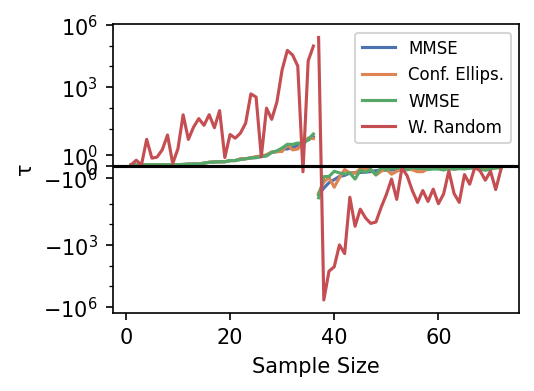
\includegraphics[width=\columnwidth]{figures/proj1/plots/LS_threshold_real/fmri_subsample_500_367_bandwidth_36_thresholds_LS.png}}
    \caption{FMRI} 
    \label{snr_FMRI}
    \end{subfigure}
    \begin{subfigure}{0.31\columnwidth}
    \resizebox{\width}{0.62\columnwidth}{
    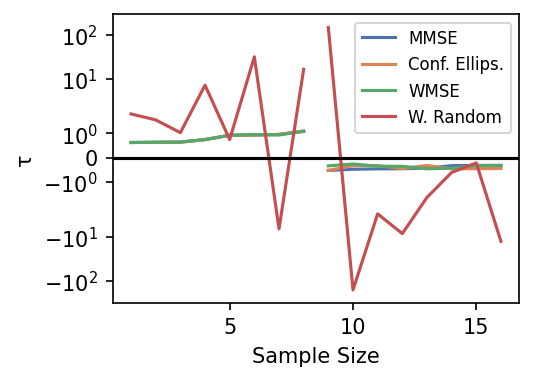
\includegraphics[width=\columnwidth]{figures/proj1/plots/LS_threshold_real/weather_45_bandwidth_8_thresholds_LS.png}}
    \caption{Weather}%
    \label{snr_Weather}%
    \end{subfigure}
    \caption{$\tau(\set{S},v)$ for real world datasets under LS and full-band noise}
\label{LS_SNR_Threshold_plots_all_real}
\end{figure}

\begin{figure}%
    \centering
    \begin{subfigure}{0.31\columnwidth}
    \resizebox{\width}{0.62\columnwidth}{
    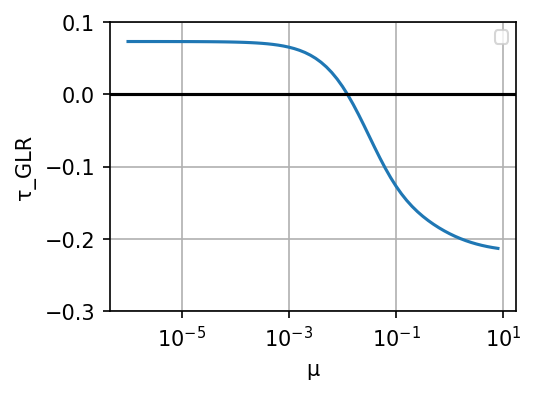
\includegraphics[width=\columnwidth]{figures/proj1/plots/GLR_threshold_real/fmri_subsample_500_GLR_threshold_fb.png}}
    \caption{FMRI}
    \label{tau_GLR_fmri}
    \end{subfigure}
    \begin{subfigure}{0.31\columnwidth}
    \resizebox{\width}{0.62\columnwidth}{
    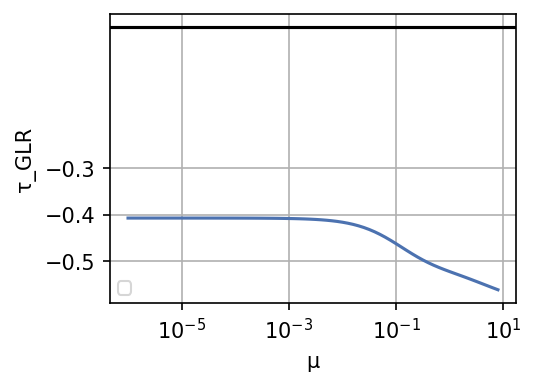
\includegraphics[width=\columnwidth]{figures/proj1/plots/GLR_threshold_real/weather_GLR_threshold_fb.png}}
    \caption{Weather}%
    \label{tau_GLR_weather}%
    \end{subfigure}
    \caption{$\tau_{GLR}$ for real world datasets}
\label{GLR_Threshold_plots_real}
\end{figure}


\begin{figure*}%
    \centering
    \begin{subfigure}{0.3\columnwidth}
    \resizebox{\width}{0.62\columnwidth}{
    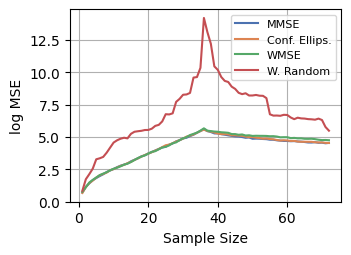
\includegraphics[width=\columnwidth]{figures/proj1/plots/LS_MSE_real/fmri_subsample_500_367_bandwidth_36_SNRdbs_-10.0_samps_72_fb_blsig_MSE_LS.png}}
    \caption{FMRI, SNR = $10^{-1}$}
    \label{fmri_MSE_subfiga}
    \end{subfigure}\hfill
    \begin{subfigure}{0.3\columnwidth}
    \resizebox{\width}{0.62\columnwidth}{
    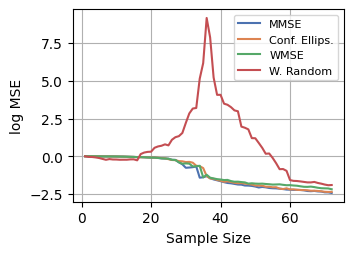
\includegraphics[width=\columnwidth]{figures/proj1/plots/LS_MSE_real/fmri_subsample_500_367_bandwidth_36_SNRdbs_20.0_samps_72_fb_blsig_MSE_LS.png}}
    \caption{FMRI, SNR = $10^{2}$}%
    \label{fmri_MSE_subfigb}%
    \end{subfigure}\hfill%
    \begin{subfigure}{0.3\columnwidth}
    \resizebox{\width}{0.62\columnwidth}{
    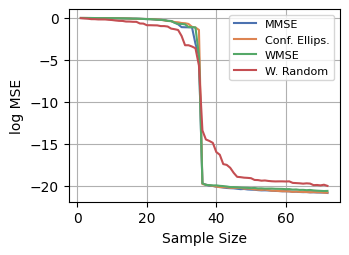
\includegraphics[width=\columnwidth]{figures/proj1/plots/LS_MSE_real/fmri_subsample_500_367_bandwidth_36_SNRdbs_100.0_samps_72_fb_blsig_MSE_LS.png}}
    \caption{FMRI, SNR = $10^{10}$}%
    \label{fmri_MSE_subfigc}%
    \end{subfigure}%
    \hfill
    \begin{subfigure}{0.3\columnwidth}
    \resizebox{\width}{0.62\columnwidth}{
    \includegraphics[width=\columnwidth]{figures/proj1/plots/LS_MSE_real/weather_45_bandwidth_8_SNRdbs_-10.0_samps_16_fb_blsig_MSE_LS.png}}
    \caption{Weather, SNR = $10^{-1}$}
    \label{weather_MSE_subfiga}
    \end{subfigure}\hfill
    \begin{subfigure}{0.3\columnwidth}
    \resizebox{\width}{0.62\columnwidth}{
    \includegraphics[width=\columnwidth]{figures/proj1/plots/LS_MSE_real/weather_45_bandwidth_8_SNRdbs_20.0_samps_16_fb_blsig_MSE_LS.png}}
    \caption{Weather, SNR = $1$}%
    \label{weather_MSE_subfigb}%
    \end{subfigure}\hfill%
    \begin{subfigure}{0.3\columnwidth}
    \resizebox{\width}{0.62\columnwidth}{
    \includegraphics[width=\columnwidth]{figures/proj1/plots/LS_MSE_real/weather_45_bandwidth_8_SNRdbs_100.0_samps_16_fb_blsig_MSE_LS.png}}
    \caption{Weather, SNR = $10^{10}$}%
    \label{weather_MSE_subfigc}%
    \end{subfigure}%
    \caption{Average MSE under LS on real world datasets and full-band noise }
\label{LS_real_MSE_fig}
\end{figure*}


We first discuss the plots of $\tau$ and $\tau_{GLR}$ for real world datasets. In practice, one cannot know for sure what the signal model of a real world signal is; however, computation of $\tau$ is dependent on our choice of theoretical signal model. We have therefore computed $\tau$ under the signal model assumptions given in Section \ref{sec:signal_model}.  
}
%By Proposition \ref{propn:averages_generalise_to_forall}, we know that there is a threshold $\tau > 0$ whenever $\tau$ is positive under our bandlimited signal model. This means that we have proven the sign of $\tau$ in \ref{LS_SNR_Threshold_plots_all_real} is correct, even though our assumption that the covariance of the signal model is $\projbl$ may not hold. We validate the accuracy of the value of our computed $\tau(\set{S},v)$ in our discussion of the MSE plots.
{\color{black}
\subsubsection{$\tau$ plots (LS)}
We examine Fig. \ref{LS_SNR_Threshold_plots_all_real}. By Proposition \ref{propn:averages_generalise_to_forall}, the sign of $\tau(\set{S},v)$ we have plotted is provably correct for \emph{any} signal model $\tau$. 
We validate the actual value of $\tau$ with MSE experiments (Figs. \ref{LS_real_MSE_fig} \& \ref{GLR_real_MSE_fig}).


\subsubsection{MSE plots (LS)}
At high noise levels, Figs. \ref{weather_MSE_subfiga} and \ref{fmri_MSE_subfiga} show a $\Lambda$-shaped MSE, validating Proposition \ref{propn:averages_generalise_to_forall} applied to Remark \ref{remark:LS_error_lambda_shaped}. 

In both plots in Fig. \ref{LS_SNR_Threshold_plots_all_real}, all of the lines are above $10^{-1}$. This corresponds to Fig. \ref{weather_MSE_subfiga} and Fig. \ref{fmri_MSE_subfiga} being $\Lambda$-shaped. In Fig. \ref{LS_SNR_Threshold_plots_all_real}, all of the lines are under $10^{10}$. This correponds to Fig. \ref{weather_MSE_subfigc} and Fig. \ref{weather_MSE_subfigc} being decreasing, which we observe.

In Fig. \ref{snr_FMRI}, we see the red line (Weighted Random sampling) is broadly above $10^2$ and the other lines (MMSE, WMSE and Confidence Ellipsoid Sampling) are below $10^2$. This corresponds to the red MSE line being $\Lambda$-shaped and the other lines decreasing in Fig. \ref{fmri_MSE_subfigb}. 

In Fig \ref{snr_Weather} all lines are below $10^{2}$ and so we expect at $\text{SNR}=10^{2}$ for all lines to be decreasing. For MMSE, WMSE and Confidence Ellipsoid sampling this is consistent with Fig. \ref{weather_MSE_subfigb}; however, it is clear our covariance assumption has underestimated $\tau$ for Weighted Random Sampling as the red line is $\Lambda$-shaped in Fig. \ref{weather_GLR_MSE_subfigb}.


We see that the real world results are broadly in line with the synthetic experiments, validating our use of the signal model presented in Section \ref{sec:signal_model} to calculate $\tau$ for LS.

\section{Discussion}
In this paper we studied the impact of sample size on linear reconstruction of noisy $k$-bandlimited graph signals. We showed theoretically and experimentally, in the same settings as much of the sample set selection literature, that reconstruction error is not always monotonic in sample size, i.e., at sufficiently low SNRs, reconstruction error can sometimes be improved by \emph{reducing} sample size. %, even if the sample set was picked by a greedy optimal sampling scheme given a fixed sample size.
Our finding reveals that existing results in the literature for the noiseless setting may not necessarily generalise to the noisy case,  even when considering regularised reconstruction methods. It also demonstrates the need to consider both optimal sample size selection and reconstruction methods at the same time, and motivates assessment of noise levels in datasets to do so. %For example, the limitation of ordinary LS reconstruction may be mitigated by regularisation schemes such as that proposed in \cite{chamon2017greedy}.
% This paper demonstrates the potential limitation of a focus on efficient optimal sample set selection, and the importance of both constructing efficient regularised reconstruction operators in reconstructing graph signals. Furthermore, it demonstrates the need for sample size bounds and guidelines specifically catering to the noisy reconstruction case with operators used in the literature, rather than optimal Bayesian operators.

\xd{One practical implication of our theoretical results is that it can provide useful guidance on how to make use of the sampling budget available. For example, if one is aware of potentially high noise present in the observed signals, to minimise MSE under LS reconstruction, it might be preferable to not use all of the provided sampling budget.}

\xd{Another use case could be a practical sampling algorithm, for both the LS and GLR reconstructions. For LS reconstruction, if one has chosen $k$ or fewer nodes by some noiseless-optimal scheme, one can calculate $\tau(\set{S},v)$ for each element of $\set{S}$, remove $v$ if $\text{SNR} < \tau(\set{S},v)$, and repeat until it is no longer possible to find a node $v$ in our remaining set $\set{S}_{rem}$ where $\text{SNR} < \tau(\set{S}_{rem},v)$.}

\xd{For the GLR reconstruction, with a fixed $\mu$ and belief that the signal model in Section \ref{sec:every_x} applies (the latter could be assessed based on past observations and is required for computation of the SNR threshold $\tau$), then our results suggest the following sampling algorithm can be considered. Given the graph structure, before observing any nodes:
\begin{enumerate}
    \item Check whether condition \ref{eq:GLR_exist_thm_B_constraint} in Theorem \ref{thm:main_GLR_exist} applies (this only depend on graph structure);
    \item If they do, compute $\tau_{GLR}$;
    \item If it is believed that $\text{SNR} < \tau_{GLR}$ holds, sample $m_{opt}$ (approximately $\sqrt{N}$) nodes at random and reconstruct from those nodes.
\end{enumerate}}

We finally remark that future work includes extending the analysis on GLR to the normalised graph Laplacian, providing bounds on $\xi_2$ for LS, analysing other graph models such as Ring graphs or studying a mode detailed ``early-stopping'' mechanism in sequential sampling schemes that do not use the full sample budget.

%%% LS plots

